\documentclass[acmsmall]{acmart}

% \acmConference
% \acmBooktitle

%\setcopyright{acmblockoption} %TODO See completed rightsreview form for your code
\setcopyright{cc}
\setcctype{by}
\acmJournal{PACMMOD}
\acmYear{2025} \acmVolume{3} \acmNumber{6 (SIGMOD)}
\acmArticle{362} \acmMonth{12}
\acmPrice{}\acmDOI{10.1145/3769827}

% Articles V3mod285-V3mod335 use
\received{April 2025}
\received[revised]{July 2025}
\received[accepted]{August 2025} 


\usepackage{amsthm}
\usepackage[shortlabels]{enumitem}
\usepackage[ruled,linesnumbered,noend]{algorithm2e}
\usepackage{cleveref}
\usepackage{subcaption} %
\graphicspath{{./plots/}}
\usepackage{thmtools}
\usepackage{etoolbox}  %

\makeatletter
\patchcmd{\@footnotetext}{\@makefntext}{\@@makefntext}{}{}
\patchcmd{\@mpfootnotetext}{\@makefntext}{\@@makefntext}{}{}
\makeatother

\settopmatter{printfolios=true}  %

\setcounter{secnumdepth}{2}

\newcommand{\Ee}{\mathcal{E}}
\newcommand{\eps}{\varepsilon}
\newcommand{\rank}{\mathrm{rank}}
\newcommand{\estRank}{\widehat{\rank}}

\newcommand{\consolidate}{\textsc{Consolidate}\xspace}


\DeclareMathOperator{\Err}{Err}


\newtheorem{theorem}{Theorem}
\newtheorem{corollary}[theorem]{Corollary}
\newtheorem{definition}[theorem]{Definition}
\newtheorem{lemma}[theorem]{Lemma}
\newtheorem{observation}[theorem]{Observation}
\newtheorem{fact}[theorem]{Fact}

\theoremstyle{remark}
\newtheorem*{remark}{Remark}


\title{SplineSketch: Even More Accurate Quantiles with Error Guarantees}


\author{Aleksander Łukasiewicz}
\orcid{0000-0003-1808-8330}
\affiliation{\institution{Computer Science Institute of Charles University}\city{Prague}\country{Czech Republic}}
\email{olekluka@iuuk.mff.cuni.cz}
    
\author{Jakub Tětek}
\orcid{0000-0002-2046-1627}
\affiliation{\institution{INSAIT, University of Sofia "St. Kliment Ohridski"}\city{Sofia}\country{Bulgaria}}
\email{j.tetek@gmail.com}



\author{Pavel Vesel{\'{y}}}
\orcid{0000-0003-1169-7934}
\affiliation{\institution{Computer Science Institute of Charles University}\city{Prague}\country{Czech Republic}}
\email{vesely@iuuk.mff.cuni.cz}


\begin{document}

\begin{abstract}
Space-efficient streaming estimation of quantiles in massive datasets is a fundamental problem with numerous applications in data monitoring and analysis. While theoretical research led to optimal algorithms, such as the Greenwald-Khanna algorithm or the KLL sketch, practitioners often use other sketches that perform significantly better in practice but lack theoretical guarantees. Most notably, the widely used $t$-digest has unbounded worst-case error.

In this paper, we seek to get the best of both worlds. We present a new quantile summary, SplineSketch, for numeric data, offering near-optimal theoretical guarantees, namely uniformly bounded rank error,  and outperforming $t$-digest by a factor of 2--20 on a range of synthetic and real-world datasets. To achieve such performance, we develop a novel approach that maintains a dynamic subdivision of the input range into buckets while fitting the input distribution using monotone cubic spline interpolation.
\end{abstract}

\keywords{quantile estimation, streaming algorithms, mergeable summaries, data sketches, cubic spline interpolation}

\begin{CCSXML}
	<ccs2012>
	<concept>
	<concept_id>10003752.10003809.10010055.10010057</concept_id>
	<concept_desc>Theory of computation~Sketching and sampling</concept_desc>
	<concept_significance>500</concept_significance>
	</concept>
	<concept>
	<concept_id>10003752.10003753.10003760</concept_id>
	<concept_desc>Theory of computation~Streaming models</concept_desc>
	<concept_significance>300</concept_significance>
	</concept>
	<concept>
	<concept_id>10003752.10010070.10010111.10011710</concept_id>
	<concept_desc>Theory of computation~Data structures and algorithms for data management</concept_desc>
	<concept_significance>300</concept_significance>
	</concept>
	</ccs2012>
\end{CCSXML}

\ccsdesc[500]{Theory of computation~Sketching and sampling}
\ccsdesc[300]{Theory of computation~Streaming models}
\ccsdesc[300]{Theory of computation~Data structures and algorithms for data management}


\maketitle




\section{Introduction}

Data sketching has become one of the main tools for dealing with massive data volumes. %
Sketches provide a scalable way to extract key features from large datasets, enabling
real-time analysis at streaming speed or massively parallel processing of distributed datasets, in applications such as network monitoring, machine learning, privacy, or bioinformatics; see %
e.g.~\cite{SifferFTL17,cormodeY20,Cormode21a,RothchildPUISB020,Smith0T20,PaghS21,baker2023genomic,bonnie2024dandd,ClemensSGH23}.

Approximating order statistics %
is a central sketching problem. %
The goal is to summarize a massive, potentially distributed dataset in a small space into a \emph{sketch} that is incrementally updatable, mergeable across data sources, and accurately approximates the data distribution.
Namely, the sketch should provide low-error estimates for the median, percentiles, and their generalization, quantiles,
and should also approximately answer rank queries -- that is, estimate the number of input items no larger than a given element.
Quantile sketches have been applied, e.g., to monitoring latencies~\cite{tene2015_latency_talk}
or for detecting anomalies~\cite{SifferFTL17}.

Streaming quantile estimation has thus received a significant attention in research community.
From the theory point of view, it has been solved to a large extent. Namely, optimal algorithms are known for the uniform error, such as the Greenwald-Khanna (GK) sketch~\cite{greenwald2001space,CormodeV20} and KLL~\cite{KarninLL16}.
However, the accuracy of these theory-based quantile summaries %
on real-world data is only a small constant factor better than the worst-case bound.
Instead, practitioners often use algorithms that perform significantly better in practice but have no guarantees.
Most notably, $t$-digest~\cite{dunning19-t-digest} is widely used --- according to~\cite{dunning21}, it has been adopted by major tech companies (reportedly Microsoft, Facebook, Google) and open-source projects (Elasticsearch \cite{::elasticdocs}, TimescaleDB \cite{::tigerdatadocumentation}, Apache Dubbo \cite{::apachedubbodocumentation}, etc.).
At the same time, no matter how large the $t$-digest is, its error can be arbitrarily bad~\cite{CormodeMRV21}.
Furthermore, to the best of our knowledge, other quantile sketches do not provide both worst-case bounds and error similar to $t$-digest in practice; see Section~\ref{sec:related}.

Here, we introduce a new quantile sketch, called SplineSketch, that not only gets the best of both worlds -- theoretical guarantees and very high accuracy in practice -- but also significantly outperforms the state of the art, including $t$-digest~\cite{dunning19-t-digest};
see Figure~\ref{figTop:error} and Section~\ref{sec:experiments}.
Our sketch processes any numerical input in a streaming fashion and is fully mergeable, enabling efficient parallel or distributed processing of large datasets.
Before explaining our contribution in more detail, we describe our setting, including the considered error guarantees.


\begin{figure}[t]
	\vspace{-0.2cm}
	\includegraphics[width=0.9\textwidth]{legend.png}
	\vspace{-0.3cm}
	\centering
	\subcaptionbox{HEPMASS dataset~\cite{hepmass}\label{fig:intro-hepmass}}{%
		\includegraphics[width=0.32\linewidth]{hepmass_average_nolegend.pdf}%
	}
	\subcaptionbox{Power dataset~\cite{individual_household_electric_power_consumption_235}\label{fig:intro-power}}{%
		\includegraphics[width=0.32\linewidth]{power_average_nolegend.pdf}%
	}
	\subcaptionbox{Books dataset~\cite{sosd,MarcusKRSMK0K20sosd}\label{fig:intro-books}}{%
		\includegraphics[width=0.32\linewidth]{sosd_books_average_nolegend.pdf}%
	}
	\caption{Average error of SplineSketch and other available sketches on three real-world datasets
		(Section~\ref{sec:experiments}).
		\vspace{-0.3cm}}
	\label{figTop:error}
\end{figure} 


\paragraph{Definitions.}
We use $n$ for the number of items currently summarized by the sketch.
For a multiset $S$ of real numbers and any $x \in \mathbb{R}$, let $\rank(x) = |\{y 
\in S : y \le x\}|$, i.e., the number of input items smaller than or equal to $x$.
For any $q \in (0,1]$, we call $y := \min \{x\in S : \rank(x) \geq q \cdot n\}$ the \emph{$q$-quantile} of $S$,
i.e., the $q$-quantile is the $\lceil q\cdot n\rceil$-th largest item in $S$ (if there are no duplicates).
This definition implies that a method for estimating ranks may be used for estimating quantiles
with the same accuracy, by performing binary search.
The \emph{aspect ratio} $\alpha$ of $S$ is defined as 
$\alpha = (\max(S) - \min(S)) / \eta$, where $\eta = \min_{i \neq j: x_i \neq x_j} |x_i - x_j|$ 
is the smallest difference of distinct items on input, assuming at least two distinct items are present.

	We focus on the \emph{streaming and mergeability settings}. The streaming model requires that the dataset $S$ is
	processed in one pass with low memory (in an arbitrary, possibly adversarial, order).
	In the more general setting of mergeable summaries~\cite{AgarwalCHPWY13},
	$S$ is arbitrarily split into a number of parts, each summarized in the streaming fashion,
	and the resulting summaries are combined via pairwise merge operations in an arbitrary way.
	In other words, besides answering rank and quantile queries,
	the sketch needs to have an update operation, which adds a new observation to the dataset,
	and a merge operation, which takes two sketches and outputs a single sketch of their combined input.

	Following a long line of work, e.g., \cite{shrivastava2004medians,greenwald2001space,AgarwalCHPWY13,KarninLL16,luo16_quantiles_experimental,CormodeV20,AssadiJPS23-GK_weighted,GuptaSW24optimaQS-non-comp,GribelyukSWY24_GK-KG_sketch},
	we study the \emph{uniform rank error}, where, for a given accuracy parameter $\eps > 0$ and any query item $x$ (that may or may not be in the input), we require
	the algorithm to return a rank estimate $\estRank(x)$ such that
	$|\estRank(x) - \rank(x)| \le \eps \cdot n$,
	and for any quantile query $q\in (0, 1]$, the algorithm should return a $q'$-quantile for $q' = q \pm \eps$.




\paragraph{Our contributions}
Our main contribution is a new technique for designing quantile summaries with bounded worst-case error and high accuracy in practice, combining dynamically maintained subdivision of the input range with a suitable interpolation
over the buckets, outlined in \Cref{sec:overview} and described in \Cref{sec:SplineSketchDescription}.

We demonstrate the power of this technique on a new quantile sketch, called SplineSketch.
It  requires a single parameter $k$ that determines its space usage, which
is $O(k)$ memory words for processing the input and $16\cdot k$ bytes when serialized for storage.
The sketch deterministically guarantees a \emph{theoretically near-optimal uniform rank error} on any input, close to the best possible error of $O(n/k)$
with $k$ memory words; namely, the error is $O(n/k \cdot \log \alpha)$,
where $\alpha$ is the aspect ratio. %
At the same time, the accuracy of our sketch in practice is in fact typically 10--200 times better than $n/k$.
Furthermore, we prove that our sketch is \emph{fully mergeable} while retaining the guarantees, i.e., we analyze it in the most general setting when the sketch is constructed by an arbitrary sequence of pairwise merge operations.
Finally, our sketch can be \emph{resized} based on the current memory requirements.



We evaluate SplineSketch in a prototype implementation and compare it with state-of-the-art sketches on a range of synthetic and real-world datasets.
We demonstrate both in the streaming and mergeability settings
that SplineSketch has error smaller by a factor of 2--20 compared to $t$-digest's error when given the same space
(see Figure~\ref{figTop:error});
in some cases, the improvement of the maximum error is by two orders of magnitude.
For an input with frequent items, a.k.a.\ heavy hitters, such accuracy is achieved by additionally using
the Misra-Gries sketch~\cite{misra1982finding} to filter them out.
The improvement over the GK~\cite{greenwald2001space} and KLL sketches~\cite{KarninLL16} is even larger, typically by 2--3 orders of magnitude.
MomentSketch~\cite{GanDTSB18} performs better on many smooth distributions as it is very compact,
but requires very large query time and its accuracy on real-world datasets is worse, without the possibility for improvement by increasing the number of moments and log-moments due to numerical issues.
We also evaluate the update, query, and merge times. Similarly to $t$-digest, we keep a buffer of size $O(k)$ when building the sketch, with bigger buffer resulting in faster update time.
Depending on the data size, we measured the average time per update of our prototype implementation to be 0.1 to 1$\mu$s, similar to $t$-digest.
Nevertheless, MomentSketch and KLL achieve 2--3 times faster update times than SplineSketch due to their simplicity.
However, the query time of SplineSketch is also 0.1 to 1$\mu$ depending on the number of queries, one of the fastest in our evaluation.
The time per merge operation in our implementation is worse than for other sketches (up to hundreds of $\mu$s) and remains to be optimized.	
Finally, we also provide ablation studies, justifying the design choices behind our sketch.

Overall, we demonstrate that besides mergeability, worst-case guarantees, and high accuracy in practice,
our approach offers flexibility, making it suitable for a range of applications.




\subsection{Overview of Our Approach}\label{sec:overview}

The core of our approach is to maintain a subdivision of the input range into \emph{buckets}
in a way that adapts well to the input distribution.
Namely, SplineSketch consists of thresholds $\tau_1, \cdots, \tau_k$ and then $(\tau_{i-1}, \tau_i]$ is the $i$-th bucket, with $\tau_0 = -\infty$.
For each bucket, we store a counter $b_i$ that represents an approximate number of items that lie in $(\tau_{i-1}, \tau_i]$;
we refer to $b_i$ as the \emph{size} of the bucket $i$.
Furthermore, we use cubic spline interpolation in order to answer queries accurately in practice;
see Figure~\ref{fig:sketch} for an illustration. %


\begin{figure}[t]
	\centering
	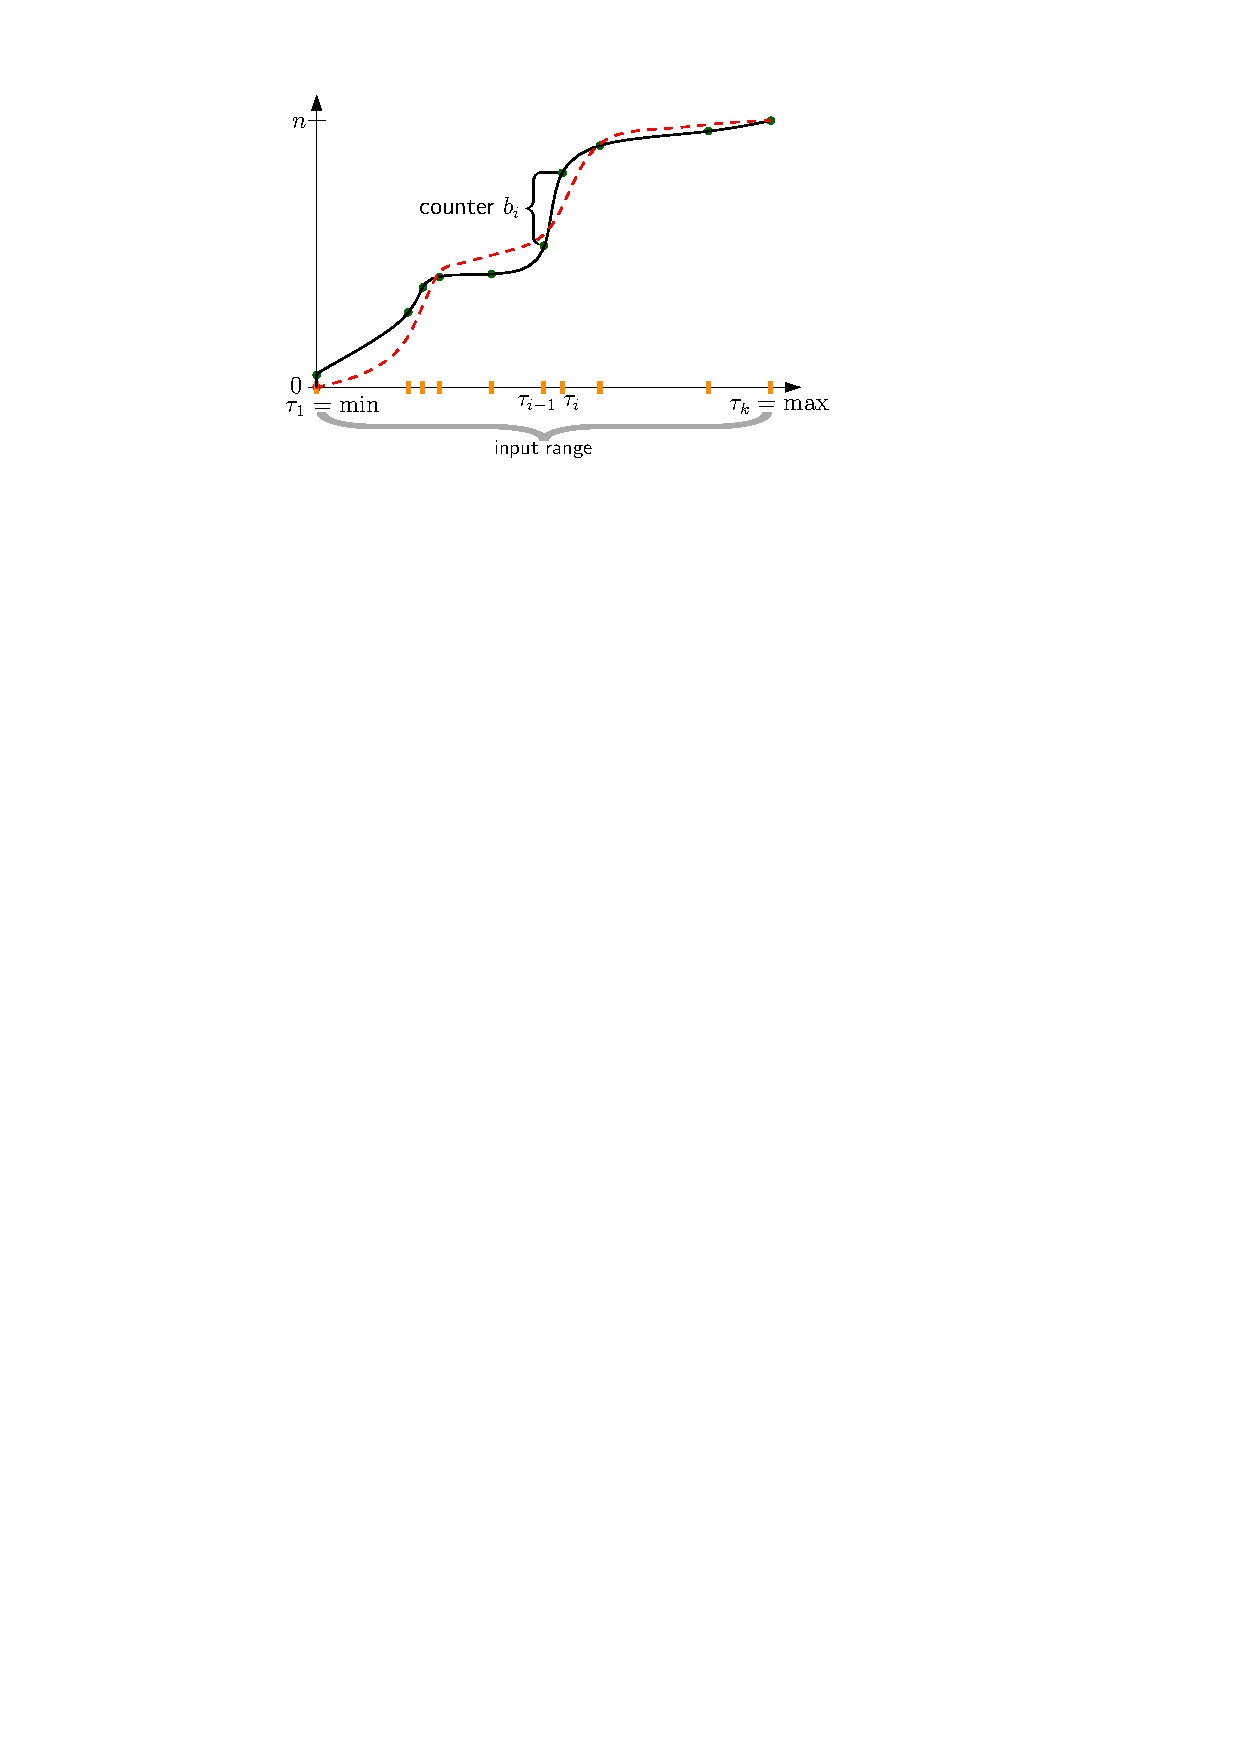
\includegraphics[width=0.5\linewidth]{buckets-spline.pdf}
	\caption{SplineSketch illustration, with the values and thresholds $\tau_i$ on the $x$ axis
	and the rank space $[0,n]$ on the $y$ axis.
	The true cumulative distribution function of the data is depicted as a red dashed curve.
	The green dots correspond to the prefix sums of bucket counters, i.e., the counter $b_i$ is the difference of the $y$ values of the green dots at $\tau_i$ and $\tau_{i-1}$.
	The solid black curve is an interpolation over the green dots.}
	\label{fig:sketch}
\end{figure}




\paragraph{Answering queries using cubic splines.}
The estimated rank of any threshold $\tau_i$ is $\sum_{j=1}^i b_i$. 
However, it is not clear what is the best way of answering rank queries that are not at one of the bucket boundaries $\tau_i$. Most of the previous work would just instead query the closest value $\tau_j$ and return that as the answer, or perform a linear interpolation. 
However, we seek to do better than that, using more advanced interpolation methods, namely the piecewise cubic Hermite interpolating polynomial (PCHIP)~\cite{fritsch.butland:1984:siamj.sci.andstat.comput., fritsch1980monotone}.
Specifically, if we are querying $x$, such that $\tau_i < x < \tau_{i+1}$, we estimate the ranks $\hat{r}_{i-1}, \cdots, \hat{r}_{i+2}$ of $\tau_{i-1}, \cdots, \tau_{i+2}$, then compute the PCHIP in order to interpolate between $\hat{r}_{i}$ and $\hat{r}_{i+1}$, and evaluate this polynomial at $x$, which gives the estimate that SplineSketch returns. 



\paragraph{Maintaining the buckets.}
The most important choice we need to make is how to set the thresholds of the buckets. 
We always set $\tau_1$ and $\tau_k$ to be the smallest and largest items seen so far, respectively. 
As new data arrives, we adjust the buckets by splitting some of them and joining certain pairs of adjacent ones.
When we \emph{join} two adjacent buckets, we simply remove the threshold they share and set the new counter to the sum of the two bucket counters.
In the \emph{split} procedure, we split the bucket in the middle. 
We then need to decide how to divide the count between the two new sub-buckets. 
To this end, we perform a query (in a way described above) at the midpoint of the original bucket and set the counts of the new sub-buckets to be consistent with the query result.
It remains to specify how we choose which buckets to split and join.
For simplicity, in the description below, we ignore the issue of update efficiency.
Ultimately, we address this by using a buffer and performing updates in batches, thereby achieving low amortized update time.


There are two rules for choosing a bucket to split.
Firstly, throughout the execution, we ensure that all buckets have counter $O(n/k)$, and we split a bucket when it gets bigger than the bound. %
We later use these size bounds, together with other invariants, to show the worst-case error bounds. 
Intuitively speaking, we show that no individual item participates in too many splits, and that each split contributes to the total error by at most the size of the bucket containing that item.

The second rule for bucket splitting is intended to achieve significantly better error in practice, while preserving the worst-case error bounds. 
To this end, for each bucket we introduce a value called the \emph{heuristic error}, which is our estimate of the order of error of the spline interpolation within the bucket.
The motivation behind this notion is that changes in the data distribution function are captured by the derivatives of that distribution.
To illustrate the intuition behind our heuristic error, suppose the data items are i.i.d.\ from an unknown distribution. 
If the growth of its CDF $F$ does not change too much around a bucket, specifically the absolute value of its second derivative $F''$ is small, the error of the spline approximation should be low as well.
In practice, we do not know the CDF and the data may not be i.i.d., but we nevertheless use an estimate of the CDF's second derivative around a bucket as a heuristic approximation of the true error.
We do not store this value explicitly and instead compute it only when needed.
If the total heuristic error can be decreased substantially by splitting one bucket and joining two other adjacent buckets, while preserving bucket bounds, then we perform the split and join of these buckets. 
The exact function that we use as the heuristic error is given by Equation~\ref{eqn:heurError-der2} in Section~\ref{sec:consolidate}.

To ensure we always have exactly $k$ buckets, whenever we split a bucket, we join some pair of adjacent buckets.
When we perform a join, we would like to choose two adjacent buckets which together would form a bucket with the lowest possible value of the heuristic error.
However, we need to ensure that the new bucket would not grow too large.
Therefore, we only consider pairs for which the size of the resulting bucket would be not too close to the bucket bound, specifically 
at most 75\% of the bucket bound.


Finally, we want to avoid performing too many joins and splits on a single bucket, as this can cause the error to accumulate.
To this end, we divide the input into epochs, where one epoch is defined as time during which the input size increased by a fixed constant factor.
If the bucket was created by a split, we mark its thresholds as \emph{protected} and we do not allow it to be joined during the same epoch.
We prove that despite all these constraints after a split there will always be at least one pair of adjacent buckets that can be joined.

\paragraph{Merging two sketches.}

The merge operation for our sketch is conceptually simple:
Given two SplineSketches on input,
we first create a combined set of thresholds by taking the union of both sketches’ thresholds,
which removes duplicates. %
We then assign counters to the new buckets based on the sum of their estimated ranks in both original sketches,
for which we use precomputed interpolations over the input sketches.
Taking the union of thresholds typically results in a sketch with more buckets than desired,
so we reduce the number of buckets by joining adjacent ones with the lowest heuristic error, until we reach the target bucket count.
To maintain worst-case guarantees, if the two sketches being merged differ significantly in size, the threshold protection from the larger sketch is preserved during merging; however, when their size is similar, we basically reset the epoch, together with the threshold protection.


\paragraph{Resizing the sketch.}
Using joining or splitting the buckets allows us to easily change the number $k$ of buckets.
Namely, when we want to make the sketch smaller, we just join an appropriate number of adjacent buckets without any splits, 
whereas for increasing the sketch size, we perform splits without joins.
The selection of buckets to split or join is done similarly as in maintaining the buckets described above.
This demonstrates the flexibility of our approach, and can be practically useful, e.g., when additional memory is allocated during input processing and the resulting sketch is later compressed to a much smaller size for storage, yielding overall better accuracy than processing directly with the smaller size.


\paragraph{Paper outline.}
\Cref{sec:related} outlines the most relevant work on quantile sketches and provides a comparison with our approach.
The full algorithmic description of SplineSketch appears in \Cref{sec:SplineSketchDescription},
together with its theoretical properties.
The implementation details appear in \Cref{sec:implementation} and the experimental evaluation in \Cref{sec:experiments}.
We conclude with discussing the pros and cons of our approach and the open problems in \Cref{sec:conclusions}.


	





\section{Related Work}\label{sec:related}

Quantile summaries are intensively investigated since the 90s, with the pioneering work of Munro and Paterson from 1978~\cite{MunroP80} who showed that exact quantile selection in the streaming setting, i.e., one pass with sublinear space, is impossible. 
In the comparison-based model, Greenwald and Khanna~\cite{greenwald2001space}
designed a deterministic algorithm, called the GK summary, that stores $O(\eps^{-1}\cdot \log \eps n)$ stream items and guarantees $\pm\, \eps\cdot n$ uniform error;
this bound is optimal among deterministic comparison-based quantile summaries~\cite{CormodeV20}.
However, the GK summary is not known to be mergeable while retaining its space bounds~\cite{AgarwalCHPWY13},
despite the fact that the intricate analysis from~\cite{greenwald2001space} was recently simplified and generalized to weighted updates~\cite{AssadiJPS23-GK_weighted,GribelyukSWY24_GK-KG_sketch}.
Randomization allows the removal of the logarithmic dependency on the stream length $n$. 
After a sequence of improvements~\cite{manku1999random,luo16_quantiles_experimental,felber2015randomized}, Karnin, Lang, and Liberty~\cite{KarninLL16} developed an optimal randomized algorithm, denoted KLL, that stores just $O(\eps^{-1})$ items (with a constant probability of a too large error).
Beyond the comparison-based model, 
$q$-digest~\cite{shrivastava2004medians} 
uses an implicit binary tree over the items' universe $\mathcal{U}$ and stores a subset of the tree nodes with associated counters.
It requires space of $O(\eps^{-1}\cdot \log |\mathcal{U}|)$ and a foreknowledge of $\mathcal{U}$.
Very recently, Gupta, Singhal, and Wu developed a compressed variant of $q$-digest that fits into $O(\eps^{-1})$ memory words, by packing more tree nodes into one memory word~\cite{GuptaSW24optimaQS-non-comp}.
However, unlike SplineSketch, GK summary, KLL, and $q$-digest do not offer practical accuracy on real-world data that goes beyond their worst-case behavior,
as demonstrated in \Cref{sec:experiments} (we only include a variant of GK and KLL as $q$-digest was already shown to be outperformed by GK in~\cite{luo16_quantiles_experimental}).

Another line of work focused on the stronger relative (multiplicative) error guarantee, which 
requires that the error for an item of rank $r$ is at most $\pm\, \eps\cdot r$.
For deterministic comparison-based algorithms,
there is a gap of $O(\log \eps n)$ between the merge-and-prune algorithm using space $O(\eps^{-1}\cdot \log^3 \eps n)$~\cite{zhangwang}
and the lower bound of $\Omega(\eps^{-1}\cdot \log^2 \eps n)$~\cite{CormodeV20}.
Efficient randomized sketches with relative error have only appeared
recently, namely, ReqSketch with space $O(\eps^{-1}\cdot \log^{1.5} \eps n)$~\cite{CormodeKLTV23} %
and its ``elastic`` version achieving space close the information-theoretic lower bound of
$\Omega(\eps^{-1}\cdot \log \eps n)$~\cite{GribelyukSWY25elasticCompactors}; however, mergeability of the ``elastic'' version is open,
while ReqSketch is analyzed in the most general mergeability setting.
There is also an extension of $q$-digest to the relative error
that uses space $O(\eps^{-1}\cdot \log \eps n\cdot \log |\mathcal{U}|)$~\cite{cormode2006space};
it is not known to be optimal.
Compared to SplineSketch, the main benefit of relative error is better accuracy for the tails which, however, comes at the cost
of higher space complexity, both in theory (additional dependency on $\log n$) and practice (see e.g.~\cite{CormodeMRV21}).
Thus, relative-error sketches are incomparable to SplineSketch and other uniform-error algorithms.
Finally, we note that stronger error guarantees, such as q-error (consider e.g. in~\cite{moerkotte2014exploiting}),
cannot be achieved in the streaming or mergeability settings with sketches of sublinear size, due to standard space lower bounds from the one-way communication complexity of indexing.

For dynamic streams (i.e., with deletions), one can only achieve the uniform error guarantee using sublinear space,
and the best quantile summary supporting deletions is Dyadic CountSketch~\cite{luo16_quantiles_experimental}.
The support for deletions comes at an additional cost of a polylogarithmic dependency on the universe size $|\mathcal{U}|$,
while insertion-only sketches, including KLL or SplineSketch, are much more space-efficient.

In contrast to rank error, DDSketch~\cite{MassonRL19} and UDDSketch~\cite{EpicocoMCPM20}
provide the relative \emph{value} error (i.e., an item close to the desired quantile in the item space)
based on maintaining a suitable exponential histogram.
While this usually captures the distribution tails well, the rank error can be arbitrarily large as these sketches in fact fail to capture most of the distribution in sufficient detail, leading to overall worse accuracy than KLL, $t$-digest, or SplineSketch.
	Furthermore, the value error is not invariant to natural data transformations such as translations.

There exist more heuristic approaches that,
similarly as SplineSketch, work only for numerical data,
but do not aim for any worst-case rank guarantees (unlike SplineSketch).
Specifically, $t$-digest~\cite{dunning19-t-digest,dunning21} performs an online one-dimensional $k$-means clustering
by averaging data items into a given number of centroids, and interpolates linearly between the centroids.
A downside of this approach is that many of the items summarized by a centroid may be smaller or larger than an adjacent centroid mean, implying under- or over-estimation.
That is, the centroids are only ordered by their means,
while the represented items may be far from ordered.
In fact, one can impose high overlaps of represented items, leading to almost arbitrarily large error on adversarial instances~\cite{CormodeMRV21}.

A different application of interpolation techniques in the context of quantile estimation was presented in~\cite{SchieferCINSW23-KLLinterpolation}.
In this work the linear interpolation were combined with the KLL sketch to improve its accuracy in some settings.

Finally, MomentSketch~\cite{GanDTSB18,MitchellFH21} is possibly the most compact summary as it consists of $k$ moments and log-moments of data items,
for a small $k$ such as $k=15$. 
Upon a query, the sketch constructs a distribution with the same moments and log-moments, using the maximum entropy principle
and Chebyshev polynomials, which is a costly operation.
The consequence is that MomentSketch only works well for certain smooth distributions but, as our experiments also demonstrate,
suffers a large error in many real-world cases,
including the uniform distribution.


The aforementioned quantile sketches form a basis for per-key quantile estimation (a simultaneous estimation of quantiles for multiple substreams in the main stream), as investigated in a recent line of work~\cite{dong.etal:2024:2024ieee40thint.conf.dataeng.icdea,guo.etal:2023:proc.29thacmsigkddconf.knowl.discov.datamin.,he.etal:2023:2023ieee39thint.conf.dataeng.icdea, shahout.etal:2023:proc.acmmanag.data}.

	Additionally, we remark that the idea of approximating the data distribution using splines has been widely used in computer science before, e.g., for query optimization~\cite{neumann.michel:2008:shar.datainf.knowl.} and indexing~\cite{kipf.etal:2020:} in database systems.





\section{Description of SplineSketch}\label{sec:SplineSketchDescription}

We provide a description of our algorithm, omitting implementation details that are explained in Section~\ref{sec:implementation}.
In fact, there are many possible implementations of the sketch that still satisfy the worst-case guarantee.
Our sketch works for any numerical input, i.e., items are integers or floating-point numbers.
We first present the algorithm assuming there are no items of high frequency, namely appearing more than $n/k$ times in the input
after inserting any number $n$ of items into SplineSketch of size $k$.
We show how to remove this assumption in Section~\ref{sec:theory}. %


\paragraph{Buckets.}
Fix an integer parameter $k \ge 6$ (a technical assumption required in the analysis).
The sketch primarily consists of $k$ distinct thresholds $\tau_1 < \tau_2 < \cdots < \tau_{k}$ and $k$ counters $b_1, \ldots, b_k$, where $b_i$ is our estimate of the number of items that lie in the interval $(\tau_{i-1}, \tau_i]$; we define $\tau_{0} = -\infty$.
We call these intervals \emph{buckets} and refer to a bucket by the index of its right threshold, so $(\tau_{i-1}, \tau_i]$ is called "bucket~$i$" or the $i$-th bucket.
We also frequently refer to $b_i$ as the \emph{size of bucket} $i$ and we define the \emph{length of bucket} $i$ as $\ell_i := \tau_i - \tau_{i-1}$.

Throughout the execution of the algorithm, we ensure that no bucket is empty
and that $\tau_1$ and $\tau_{k}$ are always set to be the minimum and the maximum item in the stream, respectively.
The latter makes the first bucket special as its counter only stores the frequency of $\tau_1$.

We also maintain a buffer of size $O(k)$ that we use for faster processing of incoming items, i.e.,
low average update time,
and one auxiliary bit-array of length $k$ for ``protected thresholds'' (Section~\ref{sec:consolidate}).
After processing the whole input, the buffer is merged into the buckets and the auxiliary bit-array can be discarded.
We ensure that all bucket counters plus the number of items in the buffer sum up to $n$.

\paragraph{Insertion and initial buckets.} When a new element arrives, we first put it in the buffer. 
When the buffer gets full, we execute the consolidate method (Section~\ref{sec:consolidate})
that may change bucket thresholds and merges the buffer into buckets. 
The only exception is the first time when the buffer gets full.
In that case, we simply sort it, pick the first and then every $\approx n / k$-th item, selecting $k$ items as the initial thresholds, and set counters $b_i$ to exactly the number of items in the corresponding buckets. 
Since no item has frequency greater than $n/k$, these selected items are distinct and every bucket is nonempty.
For the pseudocode of the bucket initialization, see Algorithm~\ref{alg:initBuckets}.

\begin{algorithm}[t] 
	\SetKwInOut{Input}{Input}
	\SetKwInOut{Output}{Output}
	\caption{Buckets Initialization}
	\label{alg:initBuckets}
	\Input{Buffer of size $n$, parameter $k$ (number of buckets)}
	\Output{Initialized $k$ buckets with thresholds $\tau_1, \dots, \tau_k$ and counters $b_1, \dots, b_k$}
	Sort all $n$ items in the buffer in ascending order\;
	For $i = 0, \dots, k -1$, pick the item at index $\min\{\lceil i\cdot (n-1) / (k-1) \rceil, n-1\}$ from the sorted buffer to form $k$ thresholds $\tau_1, \dots, \tau_k$\;
	For each bucket $(\tau_{i-1}, \tau_i]$, set the counter $b_i$ to the exact number of items in the buffer that fall into this interval\;
	Return the initialized buckets with thresholds $\tau_1, \dots, \tau_k$ and counters $b_1, \dots, b_k$\;
\end{algorithm}

\paragraph{Rank query.}
For a rank query at a threshold $\tau_i$, we return the sum of the counters up to the $i$-th, i.e., $\sum_{j=1}^i b_i$.
For $x$ strictly inside the $i$-th bucket, i.e. $\tau_{i-1} < x < \tau_i$, we use an interpolation method to estimate the rank of $x$; note that this works no matter whether $x$ appeared on input or not.
The purpose of using a suitable interpolation is to get much better error in practice,
while not affecting the worst-case bounds (see Section~\ref{sec:theory}).

Specifically, we use a monotone variant of the Piecewise Cubic Hermite Interpolating Polynomial (PCHIP)~\cite{fritsch.butland:1984:siamj.sci.andstat.comput., fritsch1980monotone}, which is an interpolation method that constructs a continuous function by fitting cubic polynomials between data points. 
Unlike standard cubic spline interpolation, PCHIP adjusts the first derivatives at each data point to preserve the shape and monotonicity of the original data.
For an introduction in greater detail, including the formulas for the interpolation, see \cite{Wong2020splines}.
Since the ranks of the input items are non-decreasing, preservation of monotonicity makes PCHIP suitable for our application.

We remark that computing this interpolation requires only the knowledge of $\tau_{i-2}, \cdots, \tau_{i+1}$ together with corresponding prefix sums of bucket counters.
Therefore, provided that we maintain the prefix sums, the computation of the interpolation takes $O(1)$ time.
The interpolation does not extrapolate, i.e., for $x < \tau_1$, it returns 0, and for $x > \tau_k$, it returns $\sum_{j=1}^k b_i$.
Since one has to find the right bucket by binary search, one query takes time $O(\log k)$  provided that the prefix sums
are precomputed.

In principle, our approach can be used with any interpolation method (ideally one that preserves monotonicity).
One popular alternative would be to use kernel smoothers.
However, this particular method would introduce additional error on the thresholds, which would be harder to control.
We leave the exploration of alternative interpolation methods for future work.
For an extensive treatment of different interpolation methods, see \cite{fan.gijbels:1996:}.

\subsection{Consolidating Buckets}\label{sec:consolidate}

The main procedure of the sketch is \consolidate. %
This method merges the buffer into the current buckets, by counting the new number of items in each bucket, and updates the counters accordingly.
It also changes the buckets based on the new values of the counters, possibly removing some of the thresholds and creating new ones.
Finally, the buffer gets emptied.
The crux of the consolidate method is how to modify the thresholds, which we describe in the remainder of this subsection.
For the pseudocode of \consolidate, see \Cref{alg:consolidate}.



\begin{figure}[t]
	\centering
	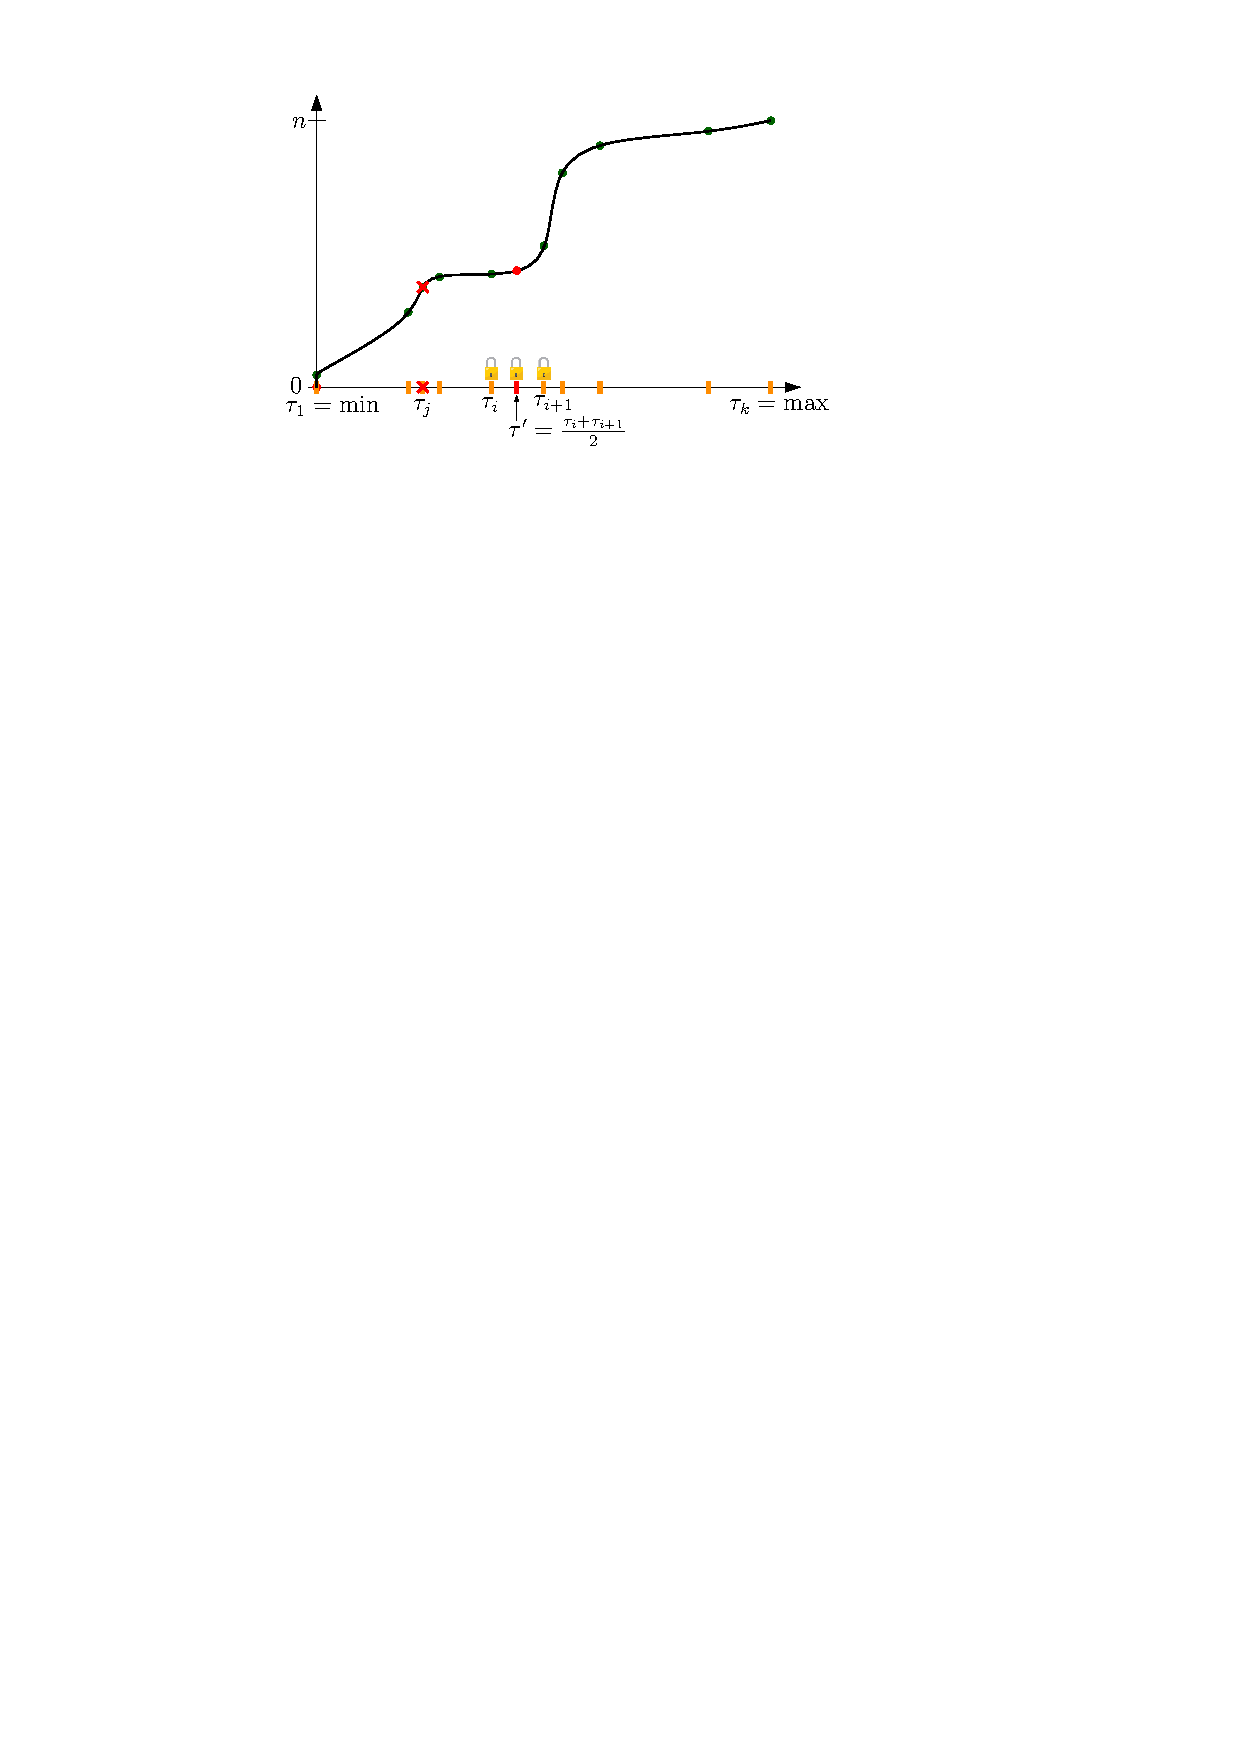
\includegraphics[width=0.5\linewidth]{buckets-joinSplit.pdf}
	\caption{Illustration of joining a pair of buckets and splitting one bucket (depicted similarly as in Figure~\ref{fig:sketch}).
		The join removes threshold $\tau_j$ and merges (sums up) the two counters of the joined buckets.
		The split takes the $i$-th bucket $(\tau_i, \tau_{i+1}]$ and inserts a new threshold $\tau'_{i+1} = (\tau_i + \tau_{i+1})/2$ in the middle,
		setting the counters of the two resulting buckets $(\tau_i, \tau'_{i+1}]$ and $(\tau'_{i+1}, \tau_{i+1}]$ using the interpolation (solid black curve).
		The thresholds $\tau_i, \tau'_{i+1}$, and $\tau_{i+1}$ get protected from joining, as depicted by the locks,
		and this protection is removed at the end of the epoch.\vspace{-0.3cm}}
	\label{fig:splitJoin}
\end{figure}

\paragraph{Joining and splitting buckets.}
We have two basic operations that change bucket thresholds, join and split (Figure~\ref{fig:splitJoin}). 
A join takes two neighboring buckets $(\tau_{i-1}, \tau_i]$ and $(\tau_{i}, \tau_{i+1}]$ for $i > 1$ and turns them into
a single bucket $(\tau_{i-1}, \tau_{i+1}]$ with its counter set to $b_i + b_{i+1}$.
Note that after joining, buckets are (implicitly) renumbered.
That is, we actually set new thresholds $\tau'$ and counters $b'$ as $\tau'_i = \tau_{i+1}$, $b'_i = b_i + b_{i+1}$, and for any $j > i$, $\tau'_j = \tau_{j+1}$ and $b'_j = b_{j+1}$.
The buckets up to $\tau_{i-1}$ do not change.

When splitting bucket $(\tau_{i-1}, \tau_i]$ for $i > 1$, we replace it by two buckets $(\tau_{i-1}, \frac{\tau_{i-1}+\tau_i}{2}]$ and $(\frac{\tau_{i-1}+\tau_i}{2}, \tau_{i}]$. The bucket counters are set as follows: We use the query method\footnote{%
	It is practical to use the query method on the buckets and buffer just before performing \consolidate\ as it may decrease the error introduced by splitting.
}
to get estimated ranks $\hat{r}$ at $\tau_{i-1}, \frac{\tau_{i-1}+\tau_i}{2},\tau_i$. We then set the counters for the two new buckets to $\hat{r}(\frac{\tau_{i-1}+\tau_i}{2}) - \hat{r}(\tau_{i-1})$ and $\hat{r}(\tau_i) - \hat{r}(\frac{\tau_{i-1}+\tau_i}{2})$, respectively.
Other buckets are again implicitly renumbered.

Observe that every split increases and every join decreases the number of buckets by one.
Thus, after every split we join some other pair of buckets, which ensures there are always $k$ buckets
(unless a change of $k$ is desired).
The crux of the algorithm lies in selecting which buckets to split and join, which we describe below.






\paragraph{Protected thresholds and epochs.}
After splitting a bucket, the estimated rank, and therefore the estimation error, at its right threshold stays the same.
However, the error at the newly created threshold may be bigger, in the worst case by the size of the original bucket counter.
If we repeatedly join and split the newly created buckets with their neighbors, we might let the error increase too much.
With the small overhead of $k$ bits when processing the input, we show how to avoid too frequent splits and joins at a single location and prevent the associated error accumulation.
To this end, we introduce the notion of \emph{protected thresholds}.

Specifically, we divide the input into \emph{epochs}. The first epoch has length $\Theta(k)$ and each successive epoch starting at time $t$ has length $0.25 \cdot t$ (we use in the analysis that the constant factor is at most $0.25$). When we split a bucket $(\tau_{i-1}, \tau_i]$, we mark all three thresholds $\tau_{i-1}, \tau'_i, \tau_i$ as protected, where $\tau'_i = (\tau_{i-1} + \tau_i)/2$ is the new threshold.
We store a bit vector of length $k$, with the $i$-th bit set to 1 when the $i$-th threshold is protected.
When a new epoch starts, we reset all thresholds to the default unprotected state
by zeroing the bit vector.
As specified later in Definition~\ref{def:joinableBuckets}, we never join buckets that have a protected threshold between them.

Note that we may still split a single bucket multiple times during one epoch,
or even during one call of \consolidate, namely, if the bucket receives many new items. Similarly, a single bucket may be joined multiple times during one consolidation.
However, a combination of splitting and then joining is not allowed -- a bucket which was created by a split cannot be joined with another bucket in the same epoch.

\paragraph{Handling new minima and maxima.}

If the buffer contains a new minimum $\tau'_1$ (an item smaller than the previous minimum $\tau_1$), we add a new bucket $(-\infty, \tau'_1]$ before all of the existing
buckets, set its counter to the frequency of $\tau'_1$ in the buffer. We also increase the counter
of the bucket $(\tau'_1, \tau_1]$ by the number of buffer items in this interval.
A new maximum $\tau'_{k}$ is handled similarly, by adding a new bucket $(\tau_{k}, \tau'_{k}]$ and setting
its counter to the number of buffer items in this interval.
For each of these at most two new buckets, we perform a join of another pair, selected according to the rules described below.
Note that these new buckets may be later split during \consolidate in which they were created, apart from the new first bucket $(-\infty, \tau'_1]$.


\paragraph{Maintaining bounds on bucket counters and small heuristic error.}

We maintain two invariants, the first of which is used to prove worst-case bounds while the second ensures high accuracy in practice.


In order to obtain a low worst-case uniform error, we need to ensure that no bucket has a too large counter.
To this end, we require that all bucket counters are bounded by $O(n/k)$, specifically
\begin{equation}\label{eqn:bucketBound}
	\forall i = 1, \dots, k:\, b_i \leq C_b \cdot n/k	
\end{equation}
for some constant $C_b > 1$
that is determined in the analysis in the full version of this paper. \footnote{Available at \url{https://arxiv.org/abs/2504.01206}.} 

Secondly, we define a \emph{heuristic error} for each bucket, which is intended to capture ``hard'' parts of the input,
where the input distribution changes a lot, namely, where the second derivative of the empirical CDF is large.
For such buckets, the PCHIP interpolation may have larger error than for buckets with a low second derivative.
Since the empirical PDF (i.e., first derivative of the CDF) in the bucket $i$ is $b_i / \ell_i$, we use the following heuristic error for bucket $i > 1$, which approximates the second derivative of the empirical CDF, normalized by length squared:
\begin{equation}\label{eqn:heurError-der2}
    \max\left(
        \frac{\left|\frac{b_i}{\ell_i} - \frac{b_{i-1}}{\ell_{i-1}}\right|}{\ell_i + \ell_{i-1}}
        \,,\,
        \frac{\left|\frac{b_{i+1}}{\ell_{i+1}} - \frac{b_i}{\ell_i}\right|}{\ell_{i+1} + \ell_i}
    \right)
    \cdot \ell_i^2.
\end{equation}
For the edge cases $i=2$ and $i=k$, we make the following assumptions: $b_{k+1} = 0$, 
$\ell_{1} = \ell_2$, and $\ell_{k+1} = \ell_{k}$; that is, we add a ``virtual'' bucket $k+1$
with zero counter and a length equal to the length of the adjacent (real) bucket, and we set the length of bucket 1 to the length of bucket 2.


We now describe how we use the bucket bound~\eqref{eqn:bucketBound} and heuristic error~\eqref{eqn:heurError-der2} when performing the splits and joins. 
Each time we split a bucket $i$, we choose a pair of adjacent buckets that do not  contain buckets created from splitting $i$, and we join the chosen pair; thus, the total number of buckets stays the same.
The pair is selected so that the bucket resulting from joining has the lowest heuristic error of all \emph{joinable pairs}, defined as follows.
In a nutshell, the bucket resulting from the join should not violate the bucket size bound~\eqref{eqn:bucketBound} or be relatively close to it.
Moreover, none of the two buckets should be subject to a split recently,
which we implement using the protected thresholds.

\begin{definition}\label{def:joinableBuckets}
    We say that a pair $i, i+1$ of adjacent buckets is \emph{joinable} if both of the following conditions hold:
    \begin{enumerate}[label=(\roman*)]
        \item the counter of the bucket resulting from the join satisfies $b_i + b_{i+1} \le 0.75\cdot C_b \cdot n/k$, and
        \item threshold $\tau_i$ is not \emph{protected}.
    \end{enumerate}
\end{definition}



We perform splits as follows. First, we take all buckets that exceed the size bound~\eqref{eqn:bucketBound}. We split them one by one, joining a joinable pair according to \Cref{def:joinableBuckets} for each split; this joinable pair is selected so that it has the lowest possible heuristic error~\eqref{eqn:heurError-der2} after temporarily performing the join (i.e., the heuristic error of a pair is computed by joining this pair without changing other buckets, then using~\eqref{eqn:heurError-der2} for the resulting bucket, and reverting the join).
In Lemma~\ref{lem:existsBucketToMerge}, we show that at least one pair of adjacent buckets is joinable.
We also join at most two further pairs of joinable buckets if the buffer contains a new minimum or maximum, each creating a new bucket.
Note that a bucket may need to be split repeatedly during one call of \consolidate, namely, if it exceeds the bucket bound~\eqref{eqn:bucketBound} substantially.

After all these necessary splits and joins, we consider a bucket $i$ with a high heuristic error~\eqref{eqn:heurError-der2}, and we split it if its error is more than $\gamma$ times greater than the lowest heuristic error of a bucket resulting from joining a joinable pair, for a parameter $\gamma > 1$ (say, $\gamma = 1.5$). Furthermore, we do not perform a split of a bucket $i$ due to the heuristic error if there are less than $k/3 + 2$ pairs of adjacent buckets that can be joined, which
is needed to prove that there is a joinable pair of buckets; see Lemma~\ref{lem:existsBucketToMerge}.
Finally, if the counter of bucket $i$ is substantially below the bound, say, $b_i \le (C_b/100) \cdot n/k$,
we also do not split bucket $i$, avoiding splitting almost empty buckets. %
We summarize the conditions for splitting:


\begin{definition}\label{def:splittableBuckets}
	We say that a bucket $i$ is \emph{splittable} if one of the following conditions holds:
	\begin{enumerate}[label=(\roman*)]
		\item bucket $i$ violates the bucket bound~\eqref{eqn:bucketBound}, i.e., $b_i > C_b\cdot n/k$, or %
		\item there are at least $k/3 + 2$ joinable pairs of buckets,
		$b_i > (C_b/100) \cdot n/k$, and the heuristic error~\eqref{eqn:heurError-der2} of bucket $i$ is $\gamma > 1$ times larger than the heuristic error of a joinable pair of buckets (after joining) not overlapping bucket $i$.
	\end{enumerate}
\end{definition}

We repeat finding a splittable bucket $i$ and a joinable pair of buckets not overlapping bucket $i$,
performing the split and join as long as there are splittable buckets.
Since every split increases the number of protected thresholds, we know that this process terminates after at most $O(k)$ iterations.
In the full version, we show it is also well-defined.
	\begin{lemma}[Lemma~B.2 in the full version]\label{lem:existsBucketToMerge}
	SplineSketch always contains a joinable pair of adjacent buckets, according to Definition~\ref{def:joinableBuckets}.
	\end{lemma}







\begin{algorithm}[h]
	\SetKwInOut{Input}{Input}
	\SetKwInOut{Output}{Output}
	\caption{\consolidate}
	\label{alg:consolidate}
	\Input{$k$ buckets and buffer of new items
	} %
	\Output{Updated buckets and protection bit vector}

	\If{$n \geq t$}{ 
		Reset protection bit vector, and set $t := 1.25 \cdot t$ \tcp*{$t$ is the end of the current epoch}
	}
	Incorporate buffer items into each bucket's counter, and empty the buffer\;
	\If{new minimum or maximum found in the buffer}{
		Add a new boundary bucket for minimum/maximum\;
		For each new bucket, join a pair of joinable buckets $j,j+1$ that has the lowest heuristic error after temporarily performing the join\;
	}
	\While{exists a splittable bucket $(\tau_{i-1}, \tau_i]$, first processing those exceeding the bound \eqref{eqn:bucketBound}}{
	   Split bucket $i$ into $(\tau_{i-1}, \tau']$ and $(\tau', \tau_i]$ for $\tau' = (\tau_i + \tau_{i-1})/2$\;
	   Mark thresholds $\tau_{i-1}, \tau', \tau_i$ as protected\;
	   Join a pair of joinable buckets $j,j+1$ that does not overlap with $(\tau_{i-1}, \tau']$ and $(\tau', \tau_i]$
	   and has the lowest heuristic error after temporarily performing the join\;
	}
	\end{algorithm}







\paragraph{Resizing the sketch during \consolidate.}
Bucket consolidation allows to change the number $k$ of buckets,
making the sketch larger or smaller as desired.
Changing from $k$ to $k'$ buckets is straightforward: 
If we increase the sketch size, i.e., $k' > k$, we perform $k' - k$ splits
without any join, first dealing with buckets exceeding bound~\eqref{eqn:bucketBound} and then in the order of the heuristic error.
On the other hand, if $k' < k$, after performing the necessary splits due to exceeding the bound (and the corresponding joins),
we execute $k - k'$ joins
in the order of their heuristic errors after joining, on bucket pairs satisfying Definition~\ref{def:joinableBuckets} and without performing any splits.
These separate splits or joins may be followed by performing \consolidate in a normal way, where we always join after splitting. %
If $k'$ is substantially different from $k$, say $|k' - k| > 0.25\cdot k$, we also %
reset the protection bit vector (otherwise, it may happen that there are no joinable pairs of buckets after resizing).

 



\subsection{Merging Two SplineSketches}\label{sec:mergeOp}

We describe how to merge two SplineSketches, $S_1$ and $S_2$, with $k_1$ and $k_2$ buckets, respectively, into a single sketch $S$ for the combined datasets.
In the analysis, we assume that  $k_1 = k_2$ but the merge operation works even for $k_1 \neq k_2$.

	
First, we create a buffer that contains all the items from the buffers of the two sketches we are merging.
Second, we take the union of all the thresholds $\tau$ from both sketches. After removing duplicates, this gives up to $k_1+k_2$ thresholds. For each of these thresholds $\tau$, we query for its rank in both input sketches and add these two ranks to get the rank of $\tau$ in the merged sketch $S$. We set the counter of each bucket to be the difference between the ranks of the endpoints.
Third, the new sketch inherits the bit vector for threshold protection from the source sketch $S_i$ that summarizes more items; that is, any threshold taken from $S_i$ remains protected if it was protected in $S_i$. However, if the total input size of the new sketch is larger than the epoch end for $S_i$, we set all thresholds to the unprotected state, starting a new epoch (in particular, if $S_1$ and $S_2$ summarize almost the same number of items, no threshold is protected after merging).

Finally, we run \consolidate that reduces the number of buckets to $k_i$ and also merges the buffer to buckets; if $k_1\neq k_2$, then the index $i$ is chosen so that the source sketch $S_i$ summarizes more items, similarly as for threshold protection (alternatively, one can also choose the larger of $k_1$ and $k_2$). Namely, we repeatedly take a joinable pair of adjacent buckets whose joining would result in a bucket with the lowest heuristic error and join it without any split until we have $k_i$ buckets.






\subsection{Theoretical Properties}\label{sec:theory}

	We now provide error bounds that hold for any input in the mergeability setting,
	which captures the streaming model (we can interpret stream updates as merges with a single-item sketch).
		\begin{theorem}[See Appendix~B.3 in the full version.]\label{thm:main}
			Suppose that we build a SplineSketch using any sequence of pairwise merge operations executed on $n$ data items, with every intermediate SplineSketch consisting of $k$ buckets.
			Then the resulting SplineSketch has a worst-case rank error of $O(\log (\alpha) \cdot n / k)$.
		\end{theorem}

The analysis assumes that no element appears more than $O(n/k)$ times.
In order to lift this assumption, we can run a heavy-hitter Misra-Gries (MG) sketch~\cite{misra1982finding} of size $O(k)$ in parallel.
We describe how to effectively combine it with SplineSketch in Section~\ref{sec:highFrequencyItems-Impl}.

We note that state-of-the-art quantile sketches achieve better worst-case accuracy-space trade-offs.
Namely, KLL using space of $O(k)$ memory words has worst-case rank error $O(n/k)$ with constant probability~\cite{KarninLL16}.
The deterministic Greenwald-Khanna (GK) sketch guarantees rank error $O(n/k)$ but with worst-case space $O(k\cdot \log (n/k))$~\cite{greenwald2001space}; the $ \log (n/k)$ factor is in general incomparable to the $\log (\alpha)$ in the error for SplineSketch.
However, both KLL and GK achieve significantly worse error in practice, as we show in Section~\ref{sec:experiments}.
As for mergeability, KLL is fully mergeable while retaining the guarantees~\cite{KarninLL16} but GK is known to be only one-way mergeable~\cite{AgarwalCHPWY13}.
Other quantile sketches have worse rank error or do not provide a bounded rank error; see Section~\ref{sec:related}.


Our analysis is very flexible with respect to the individual components and parameters of the sketch,
and allows for certain changes in constant factors (such as, e.g., the value of $C_b$ in Eqn.~\ref{eqn:bucketBound}).
Is is also completely independent of how the heuristic error is computed (and, in particular, of the value of $\gamma$ in Definition~\ref{def:splittableBuckets}).
The epochs can also be adjusted; however, our analysis requires that their lengths increase geometrically, with a factor of at most $1.25$.
As for the interpolation, it can be changed to linear or another monotone interpolation that is exact at the thresholds.
The only other property that the interpolation method must satisfy is that, in the middle of a non-empty bucket, the interpolation is bounded away from the minimum and maximum estimated values inside the bucket;
that is, a bucket counter is divided somewhat evenly during a split (a property similar to Lemma A.1 in Appendix~A of the full version).

Regarding the effect of resizing the sketch from $k'$ buckets to $k''$ buckets on the guarantees, 
the error bound of $O(\log (\alpha) \cdot n / k)$ holds with $k=\min\{k', k''\}$ after performing the resizing,
provided that no resizing was done before.
To the best of our knowledge, resizability is not addressed in the literature on quantile summaries yet.

As for the time complexities, the time for one rank or quantile query is $O(\log k)$, as derived at the beginning of Section~\ref{sec:SplineSketchDescription}.
The amortized update time can be made $O(\log k)$ by a heap-based implementation of \consolidate, as explained in Section~\ref{sec:consolidateImpl}.
Finally, the merge time is $O(k\cdot \log k)$, again for the heap-based \consolidate.
These theoretical time complexities are asymptotically the same as for KLL, GK, and $t$-digest,
albeit particular implementations of the sketches may not satisfy those theoretical bounds.



\section{Implementation Details}
\label{sec:implementation}

Here, we explain the details of our SplineSketch implementation (in Python and Java) and elaborate
on the update time. %

First, we naturally use the \texttt{double} data type (64-bit floating point numbers) for thresholds. This, however, 
implies some limitations, such as worse accuracy for some inputs with many significant digits (e.g., the SOSD benchmark~\cite{sosd,MarcusKRSMK0K20sosd}), which is due to the fact that many different items get rounded to the 
same \texttt{double} value. This can be addressed by changing the underlying data type for thresholds, e.g., to 128-bit floating-point numbers or to unsigned 64-bit integers.
Note that the internal PCHIP interpolation would still need to use floating-point numbers.


\paragraph{Quantile queries.} %
So far, we focused on answering rank queries.
In order to implement a quantile query, i.e., returning an estimated $r$-th smallest number for a given $r$,
we invert the interpolation, and query the inverse function at $r$.
This inverse exists since buckets are non-empty and the PCHIP interpolation is thus strictly increasing from $\tau_1$ to $\tau_k$.
The inverse function can be evaluated by first finding the bucket in which the inverse of $r$ lies (which can be done using binary search, assuming we maintain the prefix sums of the bucket counts). Then, inside the corresponding bucket, the value can be found numerically, for example, using Newton's method or even just bisection.
Note that our algorithm, similarly as $q$-digest~\cite{shrivastava2004medians}, may return a number that did not appear in the stream, unlike
comparison-based methods such as the KLL sketch~\cite{KarninLL16} or the Greenwald-Khanna sketch~\cite{greenwald2001space}.

\subsection{Implementations of Bucket Consolidation}
\label{sec:consolidateImpl}

We describe two particular implementations of \consolidate. The first achieves a low amortized update time,
while the second is easier to implement and works well in practice.

\vspace{-0.2cm}

\paragraph{Heap-based \consolidate.} 
To obtain an asymptotically fast \consolidate, one can use a combination of doubly-linked lists for maintaining buckets and two heaps, sorted by the bucket size and heuristic error, respectively.
This approach is formalized in the following lemma. %
Since the buffer size is $\Theta(k)$, we get $O(\log k)$ amortized complexity of an update with heap-based \consolidate\ as an immediate corollary.

\begin{restatable}{lemma}{heapBasedConsolidate}
	\label{lem:heapBasedConsolidate}
	\consolidate can be implemented in $O(k \log k)$ time.
\end{restatable}


\begin{proof}
	We maintain buckets in a doubly linked list $L$. 
	We use a queue $Q_S$ to keep track of buckets that need to be split due to violating bucket bound.
	We also use two heaps: a max-heap $H_S$ to keep track of buckets that might get split due to the heuristic error~\eqref{eqn:heurError-der2}, ordered by their heuristic errors, and a min-heap $H_J$ for joinable pairs of buckets, ordered by their heuristic errors after temporarily joining the pair.
	In both heaps, every node contains a pointer to the corresponding bucket (or pair of buckets) in $L$.
	Conversely, every bucket in $L$ contains a (constant size) list of pointers to nodes of $H_S$ and $H_J$ containing that bucket. 
	Both heaps can be initialized in $O(k)$ time.
	
	After every split and join performed by \consolidate, we update $Q_S, H_S$, and $H_J$ according to the new bucket sizes.
	Since every split and join affects only the sizes and heuristic errors of a constant number of adjacent buckets, the update can be done in $O(1)$ time using the pointers that we maintain.
	The modifications of the keys and deletions of arbitrary nodes in the heaps can be done in $O(\log k)$ time using standard decrease/increase key operation.
	
	Every split introduces a constant number of new protected thresholds and every join is accompanied with a corresponding split.
	Since the number of possible protected thresholds is bounded by $k$, the total number of splits and joins performed by \consolidate is also $O(k)$.
	Therefore, the total time complexity of the heap-based implementation of \consolidate is $O(k \log k)$.
\end{proof}


\paragraph{Iteration-based \consolidate.}
In our implementation, we use a different \consolidate that does not require linked lists or heaps.
We process the buckets in iterations such that, in each iteration, any bucket is split or joined at most once (but not both).
Since a particular bucket may need to be split or joined multiple times during \consolidate, we continue the process for multiple iterations,
until the last iteration does not change any threshold.
Throughout this process, we keep the buffer and the old buckets
for more accurate setting of counters for the new buckets.

In each iteration, we first collect the buckets with size exceeding the bound~\eqref{eqn:bucketBound} into a set $E$.
We also keep a list of splittable buckets (Definition~\ref{def:splittableBuckets}), sorted in non-increasing order by their heuristic error,
and a list of joinable pairs of buckets (Definition~\ref{def:joinableBuckets}), sorted in non-decreasing order by the resulting heuristic error after temporarily joining them.
We select $|E|$ joinable pairs according to their order that do not overlap buckets in $E$ or a previously selected joinable pairs.
Next, from the remaining buckets (not yet split or joined), we consider the splittable bucket with the largest heuristic error $h_{\mathrm{split}}$ (if any)
and the joinable pair with the lowest heuristic error $h_{\mathrm{join}}$ and if $h_{\mathrm{split}} > \gamma\cdot h_{\mathrm{join}}$ for $\gamma > 1$,
then we perform the split and join of these buckets;
in our implementation, we use $\gamma = 1.5$.
After collecting non-overlapping sets of buckets to split and join, we perform these splits and joins
in one pass over the buckets, using the buffer and interpolation over the buckets in their state before executing \consolidate
to estimate ranks in the middle of split buckets;
the usage of former buckets is important to decrease the error accumulation.
We refer to the prototypes referenced in Section~\ref{sec:experiments} for details.

Finally,
we remark that the multiplicative constant $C_b$ in the bucket bound~\eqref{eqn:bucketBound} resulting from the analysis in~Appendix~B of the full version is too large for practical usage,
and we just use $C_b = 3$, while increasing $C_b$ during an epoch if needed and resetting it to $C_b = 3$ at each epoch end. That is, if there are no joinable pairs when a bucket must be split due to exceeding the bound, we double $C_b$ and reset the iteration.
We note that such increases of $C_b$ happen rarely in practice, and provably stop after several iterations (when exceeding the constant $C_b$ from the analysis).
Therefore, this trick preserves the theoretical properties.





\subsection{Handling Frequent Items}
\label{sec:highFrequencyItems-Impl}

The theoretical error guarantees of SplineSketch, outlined in Section~\ref{sec:theory}, require 
a method for filtering items with frequency $\Omega(n/k)$.
In Section~\ref{sec:expSkewed} we show that this filtering is also important in practice, namely we provide inputs that include frequent elements and that are hard for vanilla SplineSketch.
This issue can be resolved by using a heavy hitter sketch such as the Misra-Gries (MG) summary~\cite{misra1982finding}.
However, using the MG comes at a cost of increased update, merge, and query times,
and therefore, we provide two versions of SplineSketch, with and without MG.

\vspace{-0.2cm}

\paragraph{SplineSketch with MG}

The MG sketch stores up to $k-1$ items, each with a counter $c_x$. 
When a new element $x$ arrives,
if $x$ is already in the sketch, its counter is incremented.
Otherwise, if $x$ is not in the sketch, we add it with a counter of $1$.
If adding a new item causes the sketch to reach its capacity of $k$ items, all counters are decremented.
Any item with a counter that hits zero is then removed.
It can be shown that the counters in the sketch underestimate the true frequencies by at most $n/k$.
In particular, any element with a frequency greater than $n/k$ is present in the sketch~\cite{misra1982finding}.
The MG sketch is also fully mergeable~\cite{AgarwalCHPWY13}.

In our implementation, each item $x$ in the MG sketch has an additional counter, $\hat{c}_x$, which is never decreased.
It represents the number of times $x$ has been inserted since the beginning of the stream or its last removal from the MG sketch.
During \consolidate, the MG sketch processes a buffer of new items in two stages.
First, we filter out buffer items that are present in MG and increase their sketch counters by the buffer frequencies.
For the remaining distinct items in the buffer, we process them one by one, and add them to the MG sketch with both their counters ($c_x$ and $\hat{c}_x$) set to their buffer frequency.
If at any point the MG sketch becomes full, we decrease the $c_x$ counters of all items in the MG sketch by the smallest counter.
We then remove all items with $c_x = 0$ and add them back into the buffer with frequency $\hat{c}_x$.
Finally, the items that remain in the buffer are processed by standard \consolidate.

Last, after processing the whole input, the extra space used by the MG sketch is compressed by moving all the items $x$ with frequency $\hat{c}_x < n/(2\cdot k)$
from the MG sketch to the buckets (with frequency $\hat{c}_x$). 
Additionally, if $\ell$ is the number of remaining items with $\hat{c}_x \ge n/(2\cdot k)$,
we resize SplineSketch so that there are $\max\{k - \ell, k / 2, 6\}$ buckets.
Thus, if $\ell \le k/2$, there will be $k$ buckets and MG items in total.
Based on the standard analysis of the Misra-Gries algorithm~\cite{misra1982finding}, each input element is inserted into the SplineSketch at most $n/k$ times.
To process a rank query $y$ in the MG sketch, we sum the frequencies $\hat{c}_x$ for all items $x \leq y$.
Since the values $\hat{c}_x$ are counted exactly, this sum does not increase the error of our rank estimate.
We then add the result of the SplineSketch query for $y$, i.e., the $y$'s rank estimate based on values stored in the buckets and the buffer.


\vspace{-0.2cm}

\paragraph{SplineSketch without MG}
For applications in which item frequencies are relatively small, i.e., below $n/k$,
we also implement a faster and simpler version without heavy-hitter filtering.
Still, this version tries to apply a heuristic detection of buckets with high-frequency items.
Namely, we set a lower limit on the relative length of a bucket, depending on numerical precision $\delta$ of data.
That is, a bucket $(\tau_i, \tau_{i+1}]$ must have length $\tau_{i+1} - \tau_i \ge \delta'\cdot \max\{|\tau_i|, |\tau_{i+1}|, \zeta\}$,
where $\delta' > \delta$ is a parameter and
$\zeta >0$ is the smallest non-zero absolute value of an input item ($\zeta$ is intended to avoid too small buckets around 0).
In our prototype implementations with the \texttt{double} data type, we set $\delta' = 10^{-8}$.
We do not split a bucket that would violate this relative length bound, even if it does not satisfy the size bound~\eqref{eqn:bucketBound}; this way, we avoid too many splits of a bucket with a frequent item.


We also deal with repeated thresholds when creating initial buckets in Algorithm~\ref{alg:initBuckets},
by removing thresholds that would violate the bucket length bound.
This, however, results in a sketch with less than $k$ thresholds.
We thus replace the removed thresholds by new thresholds relatively close to the previous threshold so that the resulting buckets would have length close to the relative length bound and that we end up with $k$ thresholds.
This in fact heuristically guarantees that a frequent item gets its own bucket
if it is frequent from the beginning, i.e., when creating the initial thresholds.




\section{Experimental Evaluation}\label{sec:experiments}

We have implemented SplineSketch as a prototype in Python and Java and 
compared the Java version with state-of-the-art quantile sketches for the uniform rank error
with an available implementation,
namely, $t$-digest~\cite{dunning19-t-digest}, MomentSketch~\cite{GanDTSB18}, and KLL~\cite{KarninLL16}.
Our implementation of SplineSketch and the code to run the experiments or generate the synthetic datasets,
is available at supplementary repository (\url{https://github.com/PavelVesely/SplineSketch-experiments}).
We measure the average and maximum absolute rank errors for $10^5$ evenly spaced queries,
together with average update time (or merge time if applicable) and query times.
Experiments were performed on an AMD EPYC 7302 (3 GHz) server with 251 GB RAM and SSD disk,
and run in memory, with the datasets, queries, and sketches' output stored on disk.


\vspace{-0.2cm}

\paragraph{Quantile sketches.}
We have used the Java prototype of SplineSketch, in two versions: with and without the Misra-Gries sketch.
We have also evaluated $t$-digest~\cite{dunning19-t-digest} (v3.3, \url{https://github.com/tdunning/t-digest}), MomentSketch~\cite{GanDTSB18} (\url{https://github.com/stanford-futuredata/msketch}), and KLL~\cite{KarninLL16} (Java implementation by Apache DataSketches, v6.0.0, \url{https://github.com/apache/datasketches-java}), and GKAdaptive, a practically well-performing variant of the Greenwald-Khanna sketch~\cite{greenwald2001space},
	implemented in Java according to~\cite{luo16_quantiles_experimental}.
For $t$-digest, we use the default merging variant with $k_0$ scale function that aims at the uniform error~\cite{dunning19-t-digest}.
KLL was used in the variant with the \texttt{double} data type, i.e., an instance of \texttt{KllDoublesSketch}.
We note that the MomentSketch implementation only answers quantile queries, while
our experiments required rank estimates; we have simulated rank queries using binary search
that was done for all $m$ queries in parallel in order to decrease the number of
calls to the quantile query method from $\approx m \log_2 n$ (querying just one rank) to $\approx \log_2 n$ calls (querying $m$ ranks at once), to avoid repeated computation of the distribution fitting the moments and log-moments, which is a costly operation.
We have not included other quantile sketches because they have worse error than KLL or \textit{t}\mbox{-}digest, lack available implementations (e.g., algorithms from~\cite{SchieferCINSW23-KLLinterpolation,GribelyukSWY25elasticCompactors}), or aim for different error guarantees;
namely, ReqSketch~\cite{CormodeKLTV23} provides relative rank error and its space usage is much worse than KLL's, while
the algorithmic technique is similar.
DDSketch~\cite{MassonRL19} and UDDSketch~\cite{EpicocoMCPM20} aim for the relative \emph{value} error, which captures the distribution tails
but unlike the rank error, fails to provide a reasonable approximation for most of the distribution;
indeed, we have verified that the uniform rank error of DDSketch is 10-100 times worse than KLL and even more compared to SplineSketch;
see the supplementary repository for details.

The sketch size is measured in bytes when serialized on disk for storage without supporting
data structures such as buffers. Namely, for SplineSketch and $t$-digest we count 16 bytes per bucket/centroid,
for MomentSketch we measured $16k + 16$ bytes ($k$ moments and log-moments, minimum, and maximum), for KLL we count 8 bytes per stored item,
and for GKAdaptive, we count 24 bytes per a stored tuple of one item and its rank lower and upper bounds.
For SplineSketch with MG, we also account for the MG sketch size, after removing non-frequent items from the MG and reducing the number of buckets based on the number of heavy hitters as described in Section~\ref{sec:highFrequencyItems-Impl}.

\vspace{-0.2cm}

\paragraph{Datasets.}
We use three real-world datasets, the first two from UCI Machine Learning Repository~\cite{UCI_MLrepo} : the HEPMASS dataset~\cite{hepmass} ($n = 10\,500\,000$ items from the 2nd column),
the Power dataset~\cite{individual_household_electric_power_consumption_235} ($n = 2\,075\,259$ items from the 3rd column), and the Books dataset from SOSD~\cite{sosd,MarcusKRSMK0K20sosd}.
We have synthetically generated 7 datasets by drawing i.i.d.\ (independent and identically distributed) samples from
a range of distributions: uniform, normal, Pareto, Gumbel, lognormal, loguniform, and randomly signed loguniform.
We have also generated three datasets with a distribution change, all starting with $n/2$ items from a normal distribution
and then either changing the parameters of the normal distribution (two options for the parameter change) or adding samples from a set of 42 distinct items,
which all have high frequency.
Finally, we generated a sorted input with frequent items, each with random frequency between 1 and $n/50$.
All synthetic datasets for accuracy experiments consist of $n = 10^8$ items.


Rank queries are generated by equally spaced selection from sorted data and are executed in one batch whenever possible.
While all of the sketches allow any number to be queried, using only the data points for queries leads to the same results.



%\clearpage


\begin{figure*}[t]
	\vspace{-0.2cm}
	\centering
	\includegraphics[width=0.9\textwidth]{legend.png}
	\subcaptionbox{Normal distribution\label{fig:iid-avgErr-subfig1normal}}{%
		\includegraphics[width=0.32\textwidth]{normal_logN8_average_nolegend.pdf}%
	}
	\subcaptionbox{Uniform distribution\label{fig:iid-avgErr-subfig2uniform}}{%
		\includegraphics[width=0.32\textwidth]{uniform_logN8_average_nolegend.pdf}%
	}
	\subcaptionbox{Pareto distribution\label{fig:iid-avgErr-subfigPareto}}{%
		\includegraphics[width=0.32\textwidth]{pareto_logN8_average_nolegend.pdf}%
	}
	\subcaptionbox{Lognormal distribution\label{fig:iid-avgErr-subfigLognormal}}{%
		\includegraphics[width=0.32\textwidth]{lognormal_logN8_average_nolegend.pdf}%
	}
	\subcaptionbox{Loguniform distribution\label{fig:iid-avgErr-subfigLoguniform}}{%
		\includegraphics[width=0.32\textwidth]{loguniform_logN8_average_nolegend.pdf}%
	}
		\subcaptionbox{Signed loguniform distribution\label{fig:iid-avgErr-subfigSignedLogunif}}{%
				\includegraphics[width=0.32\textwidth]{signed_loguniform_logN8_average_nolegend.pdf}%
			}
	\subcaptionbox{Signed loguniform distribution with large exponents\label{fig:iid-avgErr-subfigSignedLogunifExtreme}}{%
		\includegraphics[width=0.32\textwidth]{signed_loguniform_extreme_logN8_average_nolegend.pdf}%
	}
	\subcaptionbox{Normal distrib.\ with a small parameter change after $n/2$ items\label{fig:iid-avgErr-subfigNormalWSmallChange}}{%
		\includegraphics[width=0.32\textwidth]{normal_with_1_small_change_logN8_average_nolegend.pdf}%
	}
	\subcaptionbox{Normal distribution with a large parameter change after $n/2$ items\label{fig:iid-avgErr-subfigNormalWLargeChange}}{%
		\includegraphics[width=0.32\textwidth]{normal_with_1_large_change_logN8_average_nolegend.pdf}%
	}
	\vspace{-0.2cm} %
	\caption{Average rank error (log-scale) depending on the sketch size in bytes.
	}
	\label{fig:iid-avgErr}
\end{figure*}


\clearpage

\begin{figure*}[t]
	\vspace{-0.2cm}
	\centering
	\includegraphics[width=0.9\textwidth]{legend.png}
	\subcaptionbox{HEPMASS dataset~\cite{hepmass}\label{fig:real-maxErr-subfig1hepmass}}{%
		\includegraphics[width=0.32\textwidth]{hepmass_max_nolegend.pdf}%
	}
	\subcaptionbox{Power dataset~\cite{individual_household_electric_power_consumption_235}\label{fig:real-maxErr-subfig2power}}{%
		\includegraphics[width=0.32\textwidth]{power_max_nolegend.pdf}%
	}
	\subcaptionbox{Books dataset~\cite{sosd,MarcusKRSMK0K20sosd}\label{fig:real-maxErr-subfig2books}}{%
		\includegraphics[width=0.32\textwidth]{sosd_books_max_nolegend.pdf}%
	}
	\subcaptionbox{Normal distribution\label{fig:iid-maxErr-subfig1normal}}{%
		\includegraphics[width=0.32\textwidth]{normal_logN8_max_nolegend.pdf}%
	}
	\subcaptionbox{Uniform distribution\label{fig:iid-maxErr-subfig2uniform}}{%
		\includegraphics[width=0.32\textwidth]{uniform_logN8_max_nolegend.pdf}%
	}
	\subcaptionbox{Pareto distribution\label{fig:iid-maxErr-subfigPareto}}{%
		\includegraphics[width=0.32\textwidth]{pareto_logN8_max_nolegend.pdf}%
	}
	\subcaptionbox{Lognormal distribution\label{fig:iid-maxErr-subfigLognormal}}{%
		\includegraphics[width=0.32\textwidth]{lognormal_logN8_max_nolegend.pdf}%
	}
	\subcaptionbox{Loguniform distribution\label{fig:iid-maxErr-subfigLoguniform}}{%
		\includegraphics[width=0.32\textwidth]{loguniform_logN8_max_nolegend.pdf}%
	}
	\subcaptionbox{Signed loguniform distribution\label{fig:iid-maxErr-subfigSignedLogunif}}{%
		\includegraphics[width=0.32\textwidth]{signed_loguniform_logN8_max_nolegend.pdf}%
	}
	\subcaptionbox{Signed loguniform distribution with large exponents\label{fig:iid-maxErr-subfigSignedLogunifExtreme}}{%
		\includegraphics[width=0.32\textwidth]{signed_loguniform_extreme_logN8_max_nolegend.pdf}%
	}
	\subcaptionbox{Normal distribution with a small parameter change after $n/2$ items\label{fig:iid-maxErr-subfigNormalWSmallChange}}{%
		\includegraphics[width=0.32\textwidth]{normal_with_1_small_change_logN8_max_nolegend.pdf}%
	}
	\subcaptionbox{Normal distribution with a large parameter change after $n/2$ items\label{fig:iid-maxErr-subfigNormalWLargeChange}}{%
		\includegraphics[width=0.32\textwidth]{normal_with_1_large_change_logN8_max_nolegend.pdf}%
	}
	
	\caption{Maximum rank error (log-scale) depending on the sketch size in bytes, on a selection of datasets.
		The maximum is taken over $10^5$ evenly spaced queries.
	}
	\label{fig:iid-maxErr}
\end{figure*}

\clearpage

\subsection{Evaluation in the Streaming Setting}

\paragraph{Accuracy-space trade-off.}
We first present the results in the streaming setting, focusing on synthetic and real-world inputs without frequent items.
Figures~\ref{figTop:error} and~\ref{fig:iid-avgErr} show the average errors of the sketches depending on their size in bytes.
Figure~\ref{fig:iid-maxErr} shows the maximum error over all queries, again depending on the sketch size.
In all these plots, the error is normalized by the input size, i.e., it is the difference 
between the true rank and the estimated rank of a query item divided by the input size $n$, averaged or maximized over $10^5$ queries.
We also depict an upper bound on the theoretically optimal error bound of $O(1/k)$ in purple (loosely dotted), where $k$ is the sketch size; the hidden constant factor is based on the maximum error of KLL and GKAdaptive.

Overall, SplineSketch consistently provides the best accuracy if given sufficient size, namely $k\ge 100$,
even though in rare cases or for small sketch sizes, $t$-digest or MomentSketch are better.
In more detail,
compared to $t$-digest, SplineSketch typically achieves 2--20 times smaller error,
and in some cases, such as for normally distributed data, up to 100 times.
In a few cases, their error was similar, e.g., for the Power dataset or the maximum error for signed loguniform distribution with large exponents.
We note that the final $t$-digest size is somewhat unpredictable as
the final number of centroids does not match the compression parameter given to it, sometimes
by 66\%.
This demonstrates that $t$-digest does not use the space budget efficiently, unlike SplineSketch
which always has $k$ buckets.



MomentSketch is mainly intended for use with very small size, typically up to $k=15$ moments and log-moments,
when it often gives the best accuracy by 1--2 orders of magnitude.
It works the best on many smooth distributions (uniform, normal, loguniform, etc.).
However, its performance is significantly affected by non-smoothness as witnessed on the real-world datasets. Moreover, one cannot increase accuracy by increasing $k$ because of numeric issues.
Furthermore, MomentSketch query procedure failed with an exception on many datasets,
specifically on signed loguniform distribution with large exponents for any $k$ and 
on other datasets for large $k$.

Finally, the KLL sketch and GKAdaptive are worse than SplineSketch typically by 1--3 orders of magnitude 
as they use no interpolation (cf.~\cite{SchieferCINSW23-KLLinterpolation} for KLL with interpolation; however, no implementation is available).
Nevertheless, as KLL and GKAdaptive are comparison-based, their errors depend just on the data size and the arrival order,
not on their particular distribution, and their error decreases linearly with increasing sketch size.

We note that both versions of SplineSketch (without and with the MG sketch) provide the same accuracy on the inputs in Figures~\ref{fig:iid-avgErr} and~\ref{fig:iid-maxErr}, i.e., those without frequent items.

\paragraph{Update and query times.} %
In Figure~\ref{fig:updateTime}, we show a log-log plot with average times per update in $\mu$s
in dependence on $n$ samples from the normal distribution. The sketches' size is fixed to about 1.6 kB,
i.e., with $100$ buckets for SplineSketch and about 100 centroids for $t$-digest.
SplineSketch is evaluated without the MG sketch; see Section~\ref{sec:expSkewed} for the other version.
For MomentSketch, we use $k=15$ (i.e., size about 256 bytes) as such $k$ generally provides the best accuracy.
For KLL, we use $k=8$, i.e., the smallest meaningful size parameter.
For all sketches, the update time is decreasing fast from small data sizes
as initializing and processing the first part of the input takes relatively the most time;
namely, for SplineSketch and $t$-digest, it takes some time before the buckets/centroids stabilize.
For sufficiently long input streams, the average update time becomes constant.
As expected, MomentSketch and KLL achieve the best update times of about 0.03$\mu$s and 0.06$\mu$s, respectively.
SplineSketch achieved less than 0.1$\mu$s update time for $n\ge 10^8$,
while $t$-digest required about 0.12$\mu$.
GKAdaptive is by far the slowest for large stream lengths, with update time increasing with its size from 0.1 to 1$\mu$; see Figure~\ref{fig:updateTime2};
	however, this GKAdaptive implementation lacks running time optimization.
Figure~\ref{fig:updateTime2} shows the dependency of the update time on the sketch size.
Both SplineSketch and $t$-digest have mildly (sublinearly) increasing update time with the sketch size.
For MomentSketch, the update time is increasing linearly with its size,
while for KLL it remains stable.

\begin{figure*}[t]
	\centering
	\vspace{-0.2cm}
	\includegraphics[width=0.8\textwidth]{legendNoErrorBound.png}
	\newline
	\subcaptionbox{Log-log plot with update time depending on data size with fixed sketch size of $\approx 1.6$ kB.\label{fig:updateTime1}}{%
		\includegraphics[width=0.49\textwidth]{normal_sketchSize100_update_time_nolegend.pdf}%
	}
	\hfill
	\subcaptionbox{Update time depending on the sketch size, for $n = 10^8$.\label{fig:updateTime2}}{
		\includegraphics[width=0.49\textwidth]{normal_logN8_update_time_nolegend.pdf}
	}
	\vspace{-0.3cm}
	\caption{Time per update in $\mu$s on normally distributed data.
	}\label{fig:updateTime}
\end{figure*}
\begin{figure*}[t]
	\centering
	\subcaptionbox{Log-log plot with query time depending on the number of queries, with fixed sketch size of $\approx 1.6$ kB.\label{fig:queryTime}}{%
		\includegraphics[width=0.48\textwidth]{query_time_normal_sketchSize100_N100000000_LogLog_nolegend.pdf}%
	}
	\hfill
	\subcaptionbox{Query time depending on the sketch size for $10^5$ queries.\label{fig:queryTime2}}{%
		\includegraphics[width=0.48\textwidth]{normal_logN8_query_time_nolegend.pdf}%
	}
	\vspace{-0.4cm}
	\caption{Time per query in $\mu$s on $n=10^8$ samples from the normal distribution.
		\vspace{-0.2cm}}
\end{figure*}

In Figure~\ref{fig:queryTime}, we show average 
query times in $\mu$s depending on the number of queries in the same setup as for update time, again with a fixed sketch sizes of about 1.6 kB,
for $10^8$ normally distributed items.
KLL is the fastest to query for a large number of queries due to its simplicity, requiring only about 0.03$\mu$s per query,
while SplineSketch and GKAdaptive are nearly as fast as KLL
and outperform KLL for a small number of queries (less than 40\,000);
namely, SplineSketch and GKAdaptive use at most 1$\mu$ per query for more than 1\,000 queries.
$t$-digest is typically 2--3 times slower than SplineSketch.
MomentSketch is especially slow, by over two orders of magnitude due to the need to compute a distribution fitting the moments and also, since the particular
implementation used only provides quantile queries, we obtain rank estimates using binary search.
Figure~\ref{fig:queryTime2} shows that, with the exception of MomentSketch, the query time does not increase with the sketch size.






\subsection{Evaluation of Mergeability}\label{sec:expMerges}

	We evaluated the performance sketches when they are created by pairwise merge operations. 
	To this end, we split the input into 10\,000 chucks, feed each chunk into one sketch, and then merge the resulting
	sketches into one in a binary tree fashion, i.e., merging sketches summarizing a similar number of items.	

	As illustrated in Figures~\ref{fig:mergingAccuracy} and~\ref{fig:mergingAccuracyHepmass}, the overall accuracy picture is similar as in the streaming setting,
	with SplineSketch having 2--20 times smaller error than $t$-digest and even more compared to other sketches.
	However, the error of SplineSketch and $t$-digest got worse compared to the streaming setting, about 5--10 times,
	even though both of these sketches still largely outperform KLL and the comparison to MomentSketch is similar as in streaming.
	As for the time efficiency, we measured the time to perform a merge operation (averaged over the 9\,999 merges performed to obtain the final sketch); see Figure~\ref{fig:mergingSpeed}.
	Moment Sketch was the fastest to merge, due to taking simple sums of the moments and log-moments,
	followed by KLL, which still fit below 10$\mu$s per merge operation.
	$t$-digest and GKAdaptive required up to 100--200$\mu$s per merge, due to the need to merge the centroids,
	and SplineSketch up to 500$\mu$s as merging of buckets, while conceptually simple, requires a lot of bucket joins. 
	The query time is the same as in streaming, i.e., does not depend on how the sketch is created.
	The results for other datasets are similar; see the supplementary repository.


\begin{figure*}[t]
	\centering
		\vspace{-0.2cm}
		\includegraphics[width=0.9\textwidth]{legend.png}
		\newline
	\subcaptionbox{Maximum rank error (log-scale) on the normal distribution\label{fig:mergingAccuracy}}{%
		\includegraphics[width=0.32\textwidth]{normal_logN8_mergingM10000_max_nolegend.pdf}%
	}%
	\hfill
	\subcaptionbox{Maximum rank error (log-scale) on the HEPMASS dataset~\cite{hepmass}\label{fig:mergingAccuracyHepmass}}{%
		\includegraphics[width=0.32\textwidth]{hepmass_mergingM10000_max_nolegend.pdf}%
	}%
	\hfill
	\subcaptionbox{Time per merge operation in $\mu$s (log-scale) on the normal distribution\label{fig:mergingSpeed}}{%
		\includegraphics[width=0.32\textwidth]{normal_logN8_mergingM10000_update_time_nolegend.pdf}%
	}
	\caption{Error and merge time in the mergeability setting  depending on the sketch size in bytes,
		namely, for sketches built by merge operations from sketches for 10\,000 input chunks.
		\vspace{-0.2cm}}	
\end{figure*}

\subsection{Inputs with Heavy Hitters}\label{sec:expSkewed}

Here, we focus on inputs with high-frequency items, where SplineSketch without the MG sketch
does not perform so well.
Our results in Figures~\ref{fig:skewedAccuracy1} and~\ref{fig:skewedAccuracy2} confirm that 
using the Misra-Gries (MG) sketch alongside SplineSketch does indeed restore the very high accuracy
when the MG sketch is large enough to detect the heavy hitters (note that we account for the size of the MG sketch after compressing it as described in Section~\ref{sec:highFrequencyItems-Impl}).
In more detail, while the error of $t$-digest and SplineSketch without MG gets worse and does not improve with the sketch size,
SplineSketch with MG achieves by up to three orders of magnitude better error, and zero error
on inputs consisting of a small number of distinct items only as in Figure~\ref{fig:skewedAccuracy2}.
We note that the error of KLL and GKAdaptive remains the same as on inputs with distinct items as they are comparison-based.
As shown in Figure~\ref{fig:skewedUpdateTime}, the update time of SplineSketch with MG is about three times worse than without MG 
(though it can be optimized), while merge and query times are only slightly larger.


\begin{figure*}[htbp]
	\includegraphics[width=0.99\textwidth]{legendWithMG.png}
	\newline
	\centering
	\subcaptionbox{Average rank error (log-scale),
		on normal distribution with $n/2$ items, followed by $n/2$ high-frequency items.\label{fig:skewedAccuracy1}}{%
			\includegraphics[width=0.32\textwidth]{normal_and_distinct_42_logN8_withMG_average_nolegend.pdf}%
		}
	\hfill
	\subcaptionbox{Average rank error (log-scale),
		on a sorted input with frequent items.\label{fig:skewedAccuracy2}}{%
			\includegraphics[width=0.32\textwidth]{sorted_with_frequent_logN8_withMG_average_nolegend.pdf}%
		}
	\hfill
	\subcaptionbox{Time per update in $\mu$s for the same input as in Figure~\ref{fig:skewedAccuracy1}.\label{fig:skewedUpdateTime}}{%
			\includegraphics[width=0.32\textwidth]{normal_and_distinct_42_logN8_withMG_update_time_nolegend.pdf}%
		}
	\vspace{-0.4cm}
\caption{Accuracy and update time for inputs with frequent items, depending on the sketch size in bytes.
\vspace{-0.2cm}}	
\end{figure*}






\subsection{Ablation Studies}\label{sec:ablation}


	Here, we provide insights into the specific design choices in SplineSketch.
	First, we evaluated the benefit of using PCHIP interpolation and
	found that PCHIP interpolation achieves 3--10 times better
	error than just linear interpolation over the buckets; see Figure~\ref{fig:ablationInterpolations} for an example.

	Second, we focused on the heuristic error and compared several alternatives to the second derivative of the empirical CDF, normalized by length squared, as defined in~\eqref{eqn:heurError-der2}. The evaluated alternatives are: using no heuristic error, bucket length, bucket counter (which is the first derivative of the empirical CDF), and the third derivative of the empirical CDF, normalized by length cubed. 
	Figure~\ref{fig:ablationHeurError} shows that~\eqref{eqn:heurError-der2} is indeed the best, while using the bucket length, i.e., making the buckets similar in length on the input range, is by only about 20\% worse.
	The third derivative is about 1.5--2 times worse, and using the bucket counter or no heuristic error is over 10 times worse.

	Finally, we briefly comment on parameter tuning.
	We did not observe significant differences in the accuracy of SplineSketch with respect to parameter $\gamma > 1$ in \Cref{def:splittableBuckets} (for values between 1.1 and 2). 
	For the initial multiplicative constant $C_b$ in the bucket bound~\eqref{eqn:bucketBound},
	we tested values in $[1, 7]$ and for $C_b \ge 3$, the accuracy was similar ($C_b < 3$ was only better on the uniform distribution).
	Other parameters, such as the epoch increase factor (default=1.25) or the minimum fraction of the bucket bound in \Cref{def:splittableBuckets} of splittable buckets (default=0.01)
	also do not influence the accuracy much if adjusted. %
	See the supplementary repository for details.


\begin{figure}[htbp]
	\vspace{-0.2cm}
	\centering
	\subcaptionbox{Interpolation\label{fig:ablationInterpolations}}{
			\includegraphics[width=0.48\columnwidth]{interpolations_normal_logN8_average_legend.pdf}
		}
	\subcaptionbox{Heuristic error\label{fig:ablationHeurError}}{
			\includegraphics[width=0.48\columnwidth]{heuristicError_normal_logN8_average_legend.pdf}
		}	
	\vspace{-0.2cm}
	\caption{Ablation studies on the normal distribution.
		\vspace{-0.5cm}}
\end{figure}




\section{Conclusions and Discussion}\label{sec:conclusions}

In this work, we designed a new deterministic quantile sketch which has fixed memory consumption $O(k)$.
The main technical contribution is in careful maintenance of bucket thresholds and counters 
in order to obtain extremely accurate rank and quantile estimates, with uniformly bounded worst-case error,
achieving a near-optimal accuracy-space trade-off.
We have proven that our sketch is fully mergeable, rendering it suitable for parallel or distributed processing of massive datasets.

Besides very high accuracy on various datasets, the key advantage of our approach is flexibility.
For instance, it is possible to resize the sketch, making it smaller or larger depending on how the memory resources change
(e.g., one can use a larger sketch for input processing and then make it smaller for storage).
More importantly, if the user has a prior knowledge about the data distribution, 
it is possible to preset the initial thresholds of SplineSketch based on this prior distribution
and aim for even lower error.
Furthermore,  if the prior knowledge turns out to be wrong, our sketch adapts to the new distribution,
similarly as we have shown in Figure~\ref{fig:iid-avgErr-subfigNormalWLargeChange}.


One of the challenges when implementing SplineSketch is dealing with high-frequency items.
One possible approach is using the Misra-Gries sketch~\cite{misra1982finding}, which
	restores theoretical guarantees (Section~\ref{sec:theory})
	and very high accuracy for inputs with heavy hitters, as demonstrated in \Cref{sec:expSkewed}.
Nevertheless, using a heavy-hitter sketch comes at a cost of increased update, merge, and query times,
so we also provide a faster version without a heavy hitter sketch.
Another limitation of our implementation arises from using the \texttt{double} data type in Java,
which means that for some inputs with many significant digits (e.g., the SOSD benchmark~\cite{sosd,MarcusKRSMK0K20sosd}), accuracy degrades as the sketch rounds many items to the same \texttt{double} value;
this can be addressed by changing the underlying data type, e.g., to 64-bit integers.
While we optimized the Java version to some extent,
our implementation is so far a prototype %
intended to demonstrate the main advantages of our approach and outline its implementation challenges.
Due to the intricacies of maintaining the buckets, our sketch is slower in processing the input stream than KLL or MomentSketch,
especially when many merge operations are performed.
However, SplineSketch is already faster in streaming than $t$-digest.
However, further optimizations are possible, such as the ones presented in \cite{pfeil.etal:2025:proc.21stint.workshopdatamanag.newhardw.} (though not applicable to Python or Java).
Thus, a well-optimized implementation may be significantly faster than $t$-digest.


From the theoretical point of view, we ask whether one can modify our algorithm so that the error bounds
have better dependency on $\alpha$. We note that there is some evidence from the
comparison-based lower bounds in~\cite{CormodeV20} that a factor of $\log \log \alpha$ may be necessary
without using bit-packing tricks developed for $q$-digest in~\cite{GuptaSW24optimaQS-non-comp}.
The accuracy in practice, despite being already very high, may also be improved,
and it is not clear where is the accuracy limit of quantile summaries on real-world datasets.


Our work opens up a new direction for future work in streaming quantile estimation.
In particular, we believe that our techniques
have potential to yield much better quantile sketches with relative-error guarantees,
capturing the distribution tails more accurately than the median.
However, achieving the relative error is substantially harder as witnessed by several 
major open problems in the theory of relative-error quantile sketches (cf.~\cite{CormodeV20,GribelyukSWY25elasticCompactors}).




\paragraph{Acknowledgments.}
We thank the reviewers for their constructive feedback and suggestions for improvement.
We also thank Tomáš Domes and Jakub Komárek for their feedback.
ChatGPT was used to generate parts of this work, including polishing language in the text, pseudocodes prototyping, and translation of SplineSketch from Python to Java.
We have checked all the generated content, corrected it where necessary.
In particular, the Java implementation was largely rewritten and optimized manually.

A. Łukasiewicz and P.~Veselý were partially supported by the ERC CZ project LL2406 of the Ministry of Education of Czech Republic.
J. Tětek was supported by the VILLUM Foundation grant 16582. This research was partially funded from the Ministry of Education and Science of Bulgaria (support for INSAIT, part of the Bulgarian National Roadmap for Research Infrastructure).
P. Veselý was partially supported by Czech Science Foundation project 24-10306S
and by Center for Foundations of Modern Computer Science (Charles Univ.\ project UNCE 24/SCI/008).
Part of this work was done while A. Łukasiewicz was a PhD student at the University of Wrocław.
Part of this work was done when J. Tětek was visiting at the University of Wrocław and at Charles University. Part of this work was done while J. Tětek was employed at BARC, University of Copenhagen.


\bibliographystyle{plainnat}
\bibliography{literature}

\end{document}
